\documentclass[12pt]{report}
\usepackage[utf8]{inputenc}
\usepackage[T1]{fontenc}
\usepackage[a4paper,left=2cm,right=2cm,top=2cm,bottom=2cm]{geometry}
\usepackage[french]{babel}
\usepackage[pdftex]{graphicx}
\usepackage{enumitem}
\usepackage{listings}
\usepackage{xcolor}
\usepackage{pdfpages}
\usepackage[a4paper,left=2cm,right=2cm,top=2cm,bottom=2cm]{geometry}
\usepackage{hyperref}
\usepackage{titlesec}
\usepackage{tocloft}
\hypersetup{
	colorlinks=true,
	linkcolor=blue,
	filecolor=magenta,      
	urlcolor=cyan,
	pdftitle={Machine de Turing},
	pdfpagemode=FullScreen,
}

\setlength{\parindent}{0cm}
\setlength{\parskip}{1ex plus 0.5ex minus 0.2ex}
\newcommand{\Sharp}{{\settoheight{\dimen0}{C}C\kern-.05em \resizebox{!}{\dimen0}{\raisebox{\depth}{\#}}}}
\newcommand{\hsp}{\hspace{20pt}}
\newcommand{\HRule}{\rule{\linewidth}{0.5mm}}

\definecolor{codegreen}{rgb}{0,0.6,0}
\definecolor{codegray}{rgb}{0.5,0.5,0.5}
\definecolor{codepurple}{rgb}{0.58,0,0.82}
\definecolor{backcolour}{rgb}{0.95,0.95,0.92}

\lstdefinestyle{mystyle}{
	backgroundcolor=\color{backcolour},   
	commentstyle=\color{codegreen},
	keywordstyle=\color{magenta},
	numberstyle=\tiny\color{codegray},
	stringstyle=\color{codepurple},
	basicstyle=\ttfamily\footnotesize,
	breakatwhitespace=false,         
	breaklines=true,                 
	captionpos=b,                    
	keepspaces=true,                 
	numbers=left,                    
	numbersep=5pt,                  
	showspaces=false,                
	showstringspaces=false,
	showtabs=false,                  
	tabsize=2
}

\lstset{style=mystyle}

\titleformat{\chapter}[block]
{\normalfont\huge\bfseries}{}{0pt}{}

\title{Machine de Turing}
\author{ALLEGRE--COMMINGES Clément et BROUARD Romain}
\date{~}
\begin{document}
	\maketitle
	\tableofcontents
	\chapter{Introduction}
	\section{Un peu d'histoire...}
	En 1928, Le mathématicien allemand David Hilbert énonce le "problème de la décision". Il se demande s'il est possible de trouver une méthode « effectivement calculable » pour décider si une proposition est démontrable. Pour résoudre ce problème, il faut caractériser ce qu'est un procédé effectivement calculable. C'est alors qu'Alan Turing, alors en thèse à Cambridge, conceptualise une machine universelle et prouve grâce à cette dernière que le problème de l'arrêt est indécidable, ce qui permet de donner une réponse négative au problème d'Hilbert pour l'arithmétique. C'est alors qu'Alan Turing introduit les concepts de programme et programmation.\\
	Ce concept de machine universelle, que nous appellerons désormais Machine de Turing Universelle (MTU) n'est pas réalisable puisqu'il s'agit d'un objet mathématique, dont on va détailler le fonctionnement plus tard. Néanmoins, une Machine de Turing à état fini peut-être construite, et la première vit donc le jour à Bletchley Park pendant la Seconde Guerre Mondiale, où Turing lui-même et une équipe de scientifique triés sur le volet par le MI6\footnote{Services de renseignement britanniques} construisirent une Machine de Turing pour casser les codes allemands générés par la machine Enigma. \cite{mtu_wikip}\\
	
	\section{Fonctionnement d'une MTU}
	Une MTU se compose de quatre éléments essentiels :
	\begin{itemize}[label=$-$]
		\item un ruban de taille infinie, divisé en cases.
		\item une tête de lecture/écriture (qu'on appellera simplement tête de lecture, même si elle permet également d'écrire sur le ruban)
		\item un état interne
		\item une table de transition.
	\end{itemize}
	Une machine de Turing traite des symboles. L'ensemble des symboles est appelé Alphabet.\\
	Le ruban permet d'accueillir des symboles qui seront lus et écrits par la tête de lecture.\\
	La tête de lecture permet de lire et écrire un symbole. Elle peut se déplacer vers la gauche ou la droite.\\
	\\
	Une machine de Turing fonctionne donc de la manière suivante :
	\begin{enumerate}
		\item La tête de lecture lit le symbole qu'elle pointe sur le ruban.
		\item En fonction de son état et du symbole lu, la tête de lecture écrit un symbole à la place de celui qu'elle a lu précédemment.
		\item Un déplacement est  choisi en fonction de l'état de la tête de lecture et du symbole lu.
		\item La tête de lecture change d'état.
		\item Le ruban se déplace vers la droite ou vers la gauche selon le déplacement choisi précédemment.
		\item Puis on recommence depuis le 1.
	\end{enumerate}
	 On peut donc résumer le fonctionnement comme cela : à chaque "cycle", on choisi un symbole à écrire, un nouvel état pour la tête de lecture, et un déplacement, en fonction d'un symbole lu et de l'état actuel. On peut donc définir une fonction de transition, qui va se charger de déterminer l'état futur d'une MTU en fonction de ton état courant. L'ensemble des fonctions de transition permettant de traiter un "mot" peut être représenté sous la forme d'une table de transitions ou d'un graphe de transitions.\\
	 Un mot traité est dit accepté si une Machine de Turing s'arrête en état final après l'avoir intégralement traité.\\
	 Une MTU possède forcément un nombre fini d'états, et elle a au moins deux états obligatoires : $q_O$ l'état initial, et $F$ un ensemble d'états d'acceptation.\\
	 \\
	 Une machine de Turing est donc définie par :\\
	 \begin{itemize}[label=$-$]
	 	\item $Q$ un ensemble fini d'états.\\
	 	\item $q_0$ un état initial tel que $q_0 \in Q$.\\
	 	\item $F$ un ensemble d'états d'acceptation tel que $F \subseteq Q$.\\
	 	\item $\Gamma$ un ensemble fini de symboles.\\
	 	\item $\Sigma$ un ensemble fini de symboles d'entrée tel que $\Sigma \subseteq \Gamma$.\\
	 	\item $B$ un symbole de ruban vide tel que $B \in \Gamma \setminus \Sigma$.
	 	\item $\delta$ une fonction de transition.\\
	\end{itemize}
	 Une fonction de transition se formalise donc comme ceci :\\
	 \[ \delta (q, Z) \to (p, Y, D) \]
	 avec $q$ l'état de la tête de lecture, $Z$ le symbole pointé, $p$ le nouvel état, $Y$ le nouveau symbole et $D$ le déplacement. \cite{mt_wikip}\\
	 \\
	 Exemple d'une table de transition pour une Machine de Turing acceptant le langage $L = \lbrace a^kb^k \, \vert \, k > 0 \rbrace$ avec $q_0$ comme état initial (représenté par une $\to$), et $q_4$ comme état d'acceptation (représenté par $\ast$):\\
	 \\
	 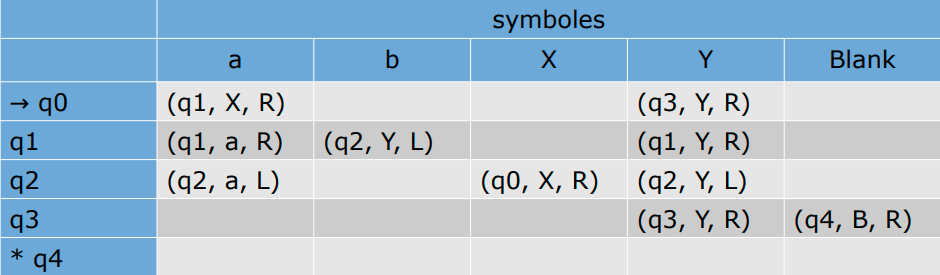
\includegraphics[width=\textwidth]{img/fig1}
	 \\
	 \\
	 Le but de ce projet va donc être de concevoir une Machine de Turing électronique fonctionnant tel que défini ci-dessus.
	 \chapter{Reprise de l'existant}
	 Le projet Machine de Turing se base sur un système existant dans le commerce. Le but est de concevoir une machine avec des fonctionnalités se rapprochant de ce modèle existant.\cite{site_mtu_fr} \\
	 Ce projet avait déjà été donné l'an passé, et nous avons eu accès à l'analyse et la maquette produite par le groupe qui s'en était chargé.\\
	 Leur maquette fonctionne, elle se compose de 8 boutons poussoirs, d'un micro-contrôleur PIC24FJ64GA002, et de deux matrices de LEDs SparkFun communiquant en SPI.\\
	 Nous avons trouvé que leur travail pouvait être amélioré, et nous avons proposé un cahier des charges ambitieux au client. Le travail d'analyse effectué l'an passé correspondait à peu près à la partie 1 de notre cahier des charges, c'est pourquoi nous avons décidé de rajouter deux autres parties, pour nous rapprocher le plus possible du système modèle.
	 \chapter{Conception}
	 \section{Cahier des charges}
	 Le cahier des charges est composé de trois parties. La partie 1 doit être traitée absolument, les parties 2 et 3 seront traitées si le temps nous le permet.
	 \subsection{Partie 1}
	 Dans un premier temps, le système conçu doit être capable de :
	 \begin{itemize}[label=$-$]
	 	\item exécuter un programme prédéfini (codé en dur dans le programme microcontrôleur).
	 	\item avoir un mode pas à pas pour l'exécution du programme.
	 	\item avoir un mode continu pour l'exécution du programme.
	 	\item gérer l'affichage de l'état du ruban.
	 	\item gérer l'affichage de la position de la tête de lecture.
	 	\item gérer l'affichage de la table de transition.
	 \end{itemize}
	 \subsection{Partie 2}
	 Dans un second temps, il faut rajouter :
	 \begin{itemize}[label=$-$]
	 	\item  la possibilité de sélectionner un programme via un menu.
	 	\item le stockage des programmes à sélectionner.
	 	\item l'initialisation manuelle du ruban et de la position de la tête de lecture.
	 \end{itemize}
	 \subsection{Partie 3}
	 Enfin pour obtenir un système complet, il faut implémenter :
	 \begin{itemize}[label=$-$]
	 	\item la programmation directement sur la machine d'une table de transition.
	 	\item l'enregistrement de la table de transition programmée dans le support de stockage.
	 	\item un reset de la programmation de la ligne en cours.
	 	\item l'affichage d'une description du programme.
	 \end{itemize}
 	\section{Définition des besoins}
 	 \subsection{Diagramme bête à corne}
 	 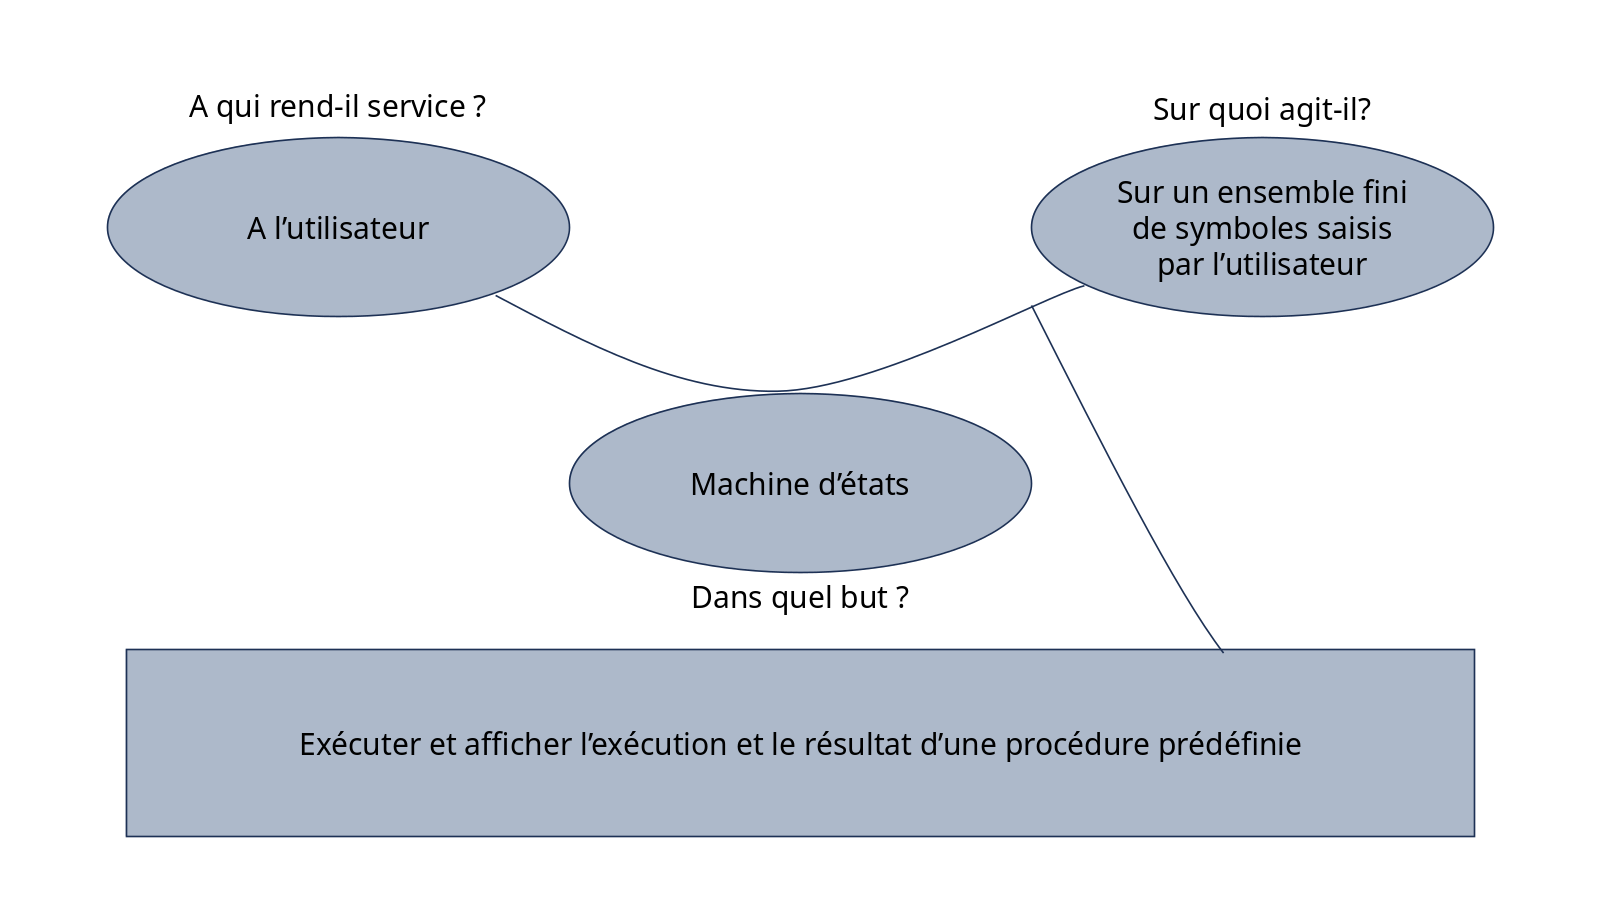
\includegraphics[width=\textwidth]{img/bete_a_corne}
 	 \subsection{Matrice Moscow}
 	 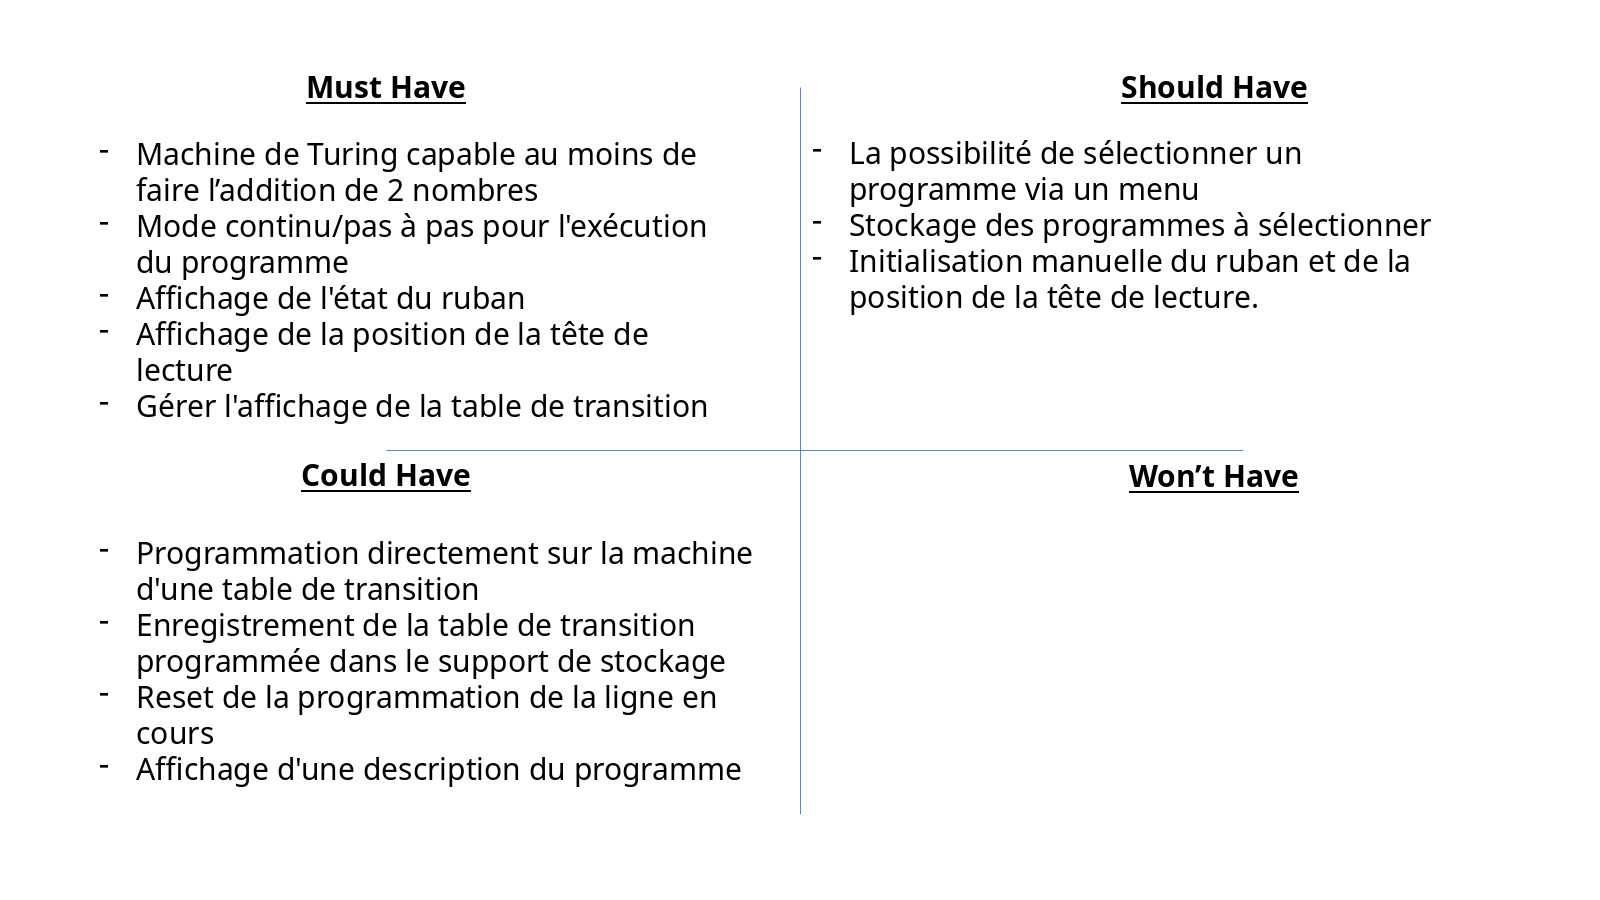
\includegraphics[width=\textwidth]{img/moscow}
	 \section{Conception Matérielle}
	 Pour concevoir notre système, nous avons décidé de traiter les trois parties en même temps, ce qui nous évite de devoir repasser par une phase de conception et d'adaptation lors de la réalisation des parties 2 et 3.\\
	 \subsection{SFN1}
	 Nous avons donc commencé par dessiner un Schéma fonctionnel de premier niveau, pour définir les différentes entrées et sorties de notre système :\\
	 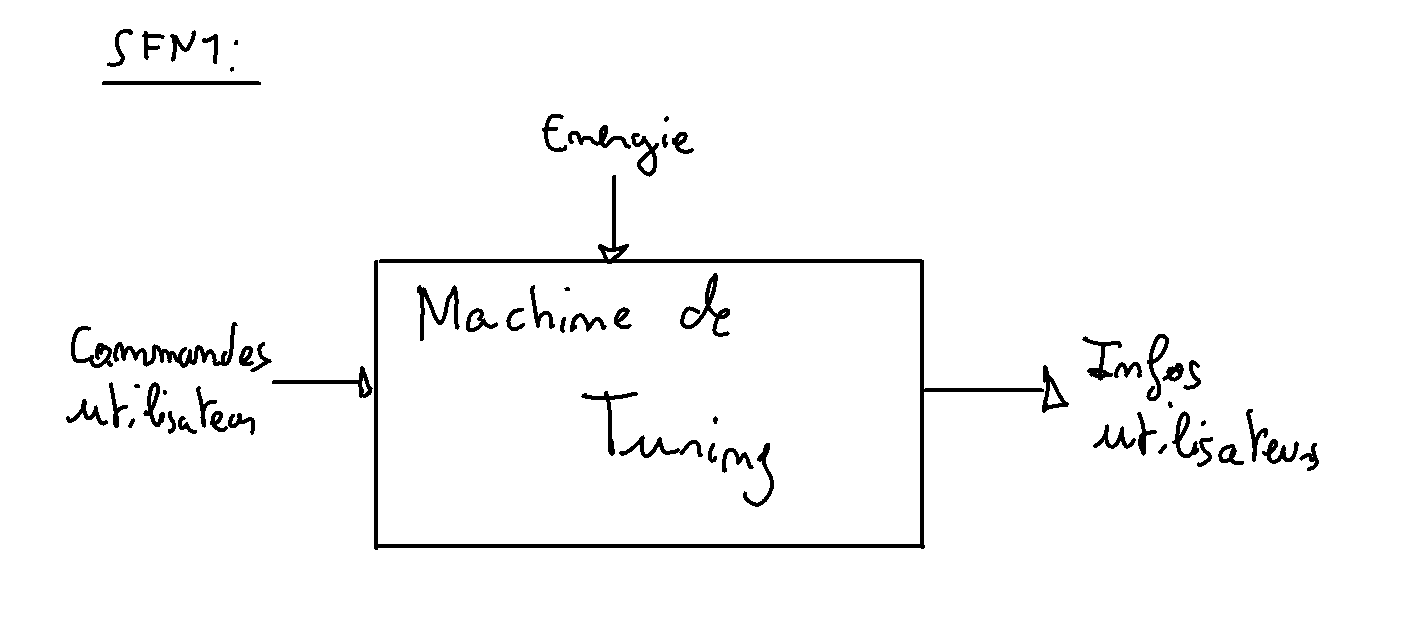
\includegraphics[width=\textwidth]{img/SFN1}
	\subsection{SFnD}
	On peut désormais rentrer un peu plus dans le détail avec un SF1D :\\
	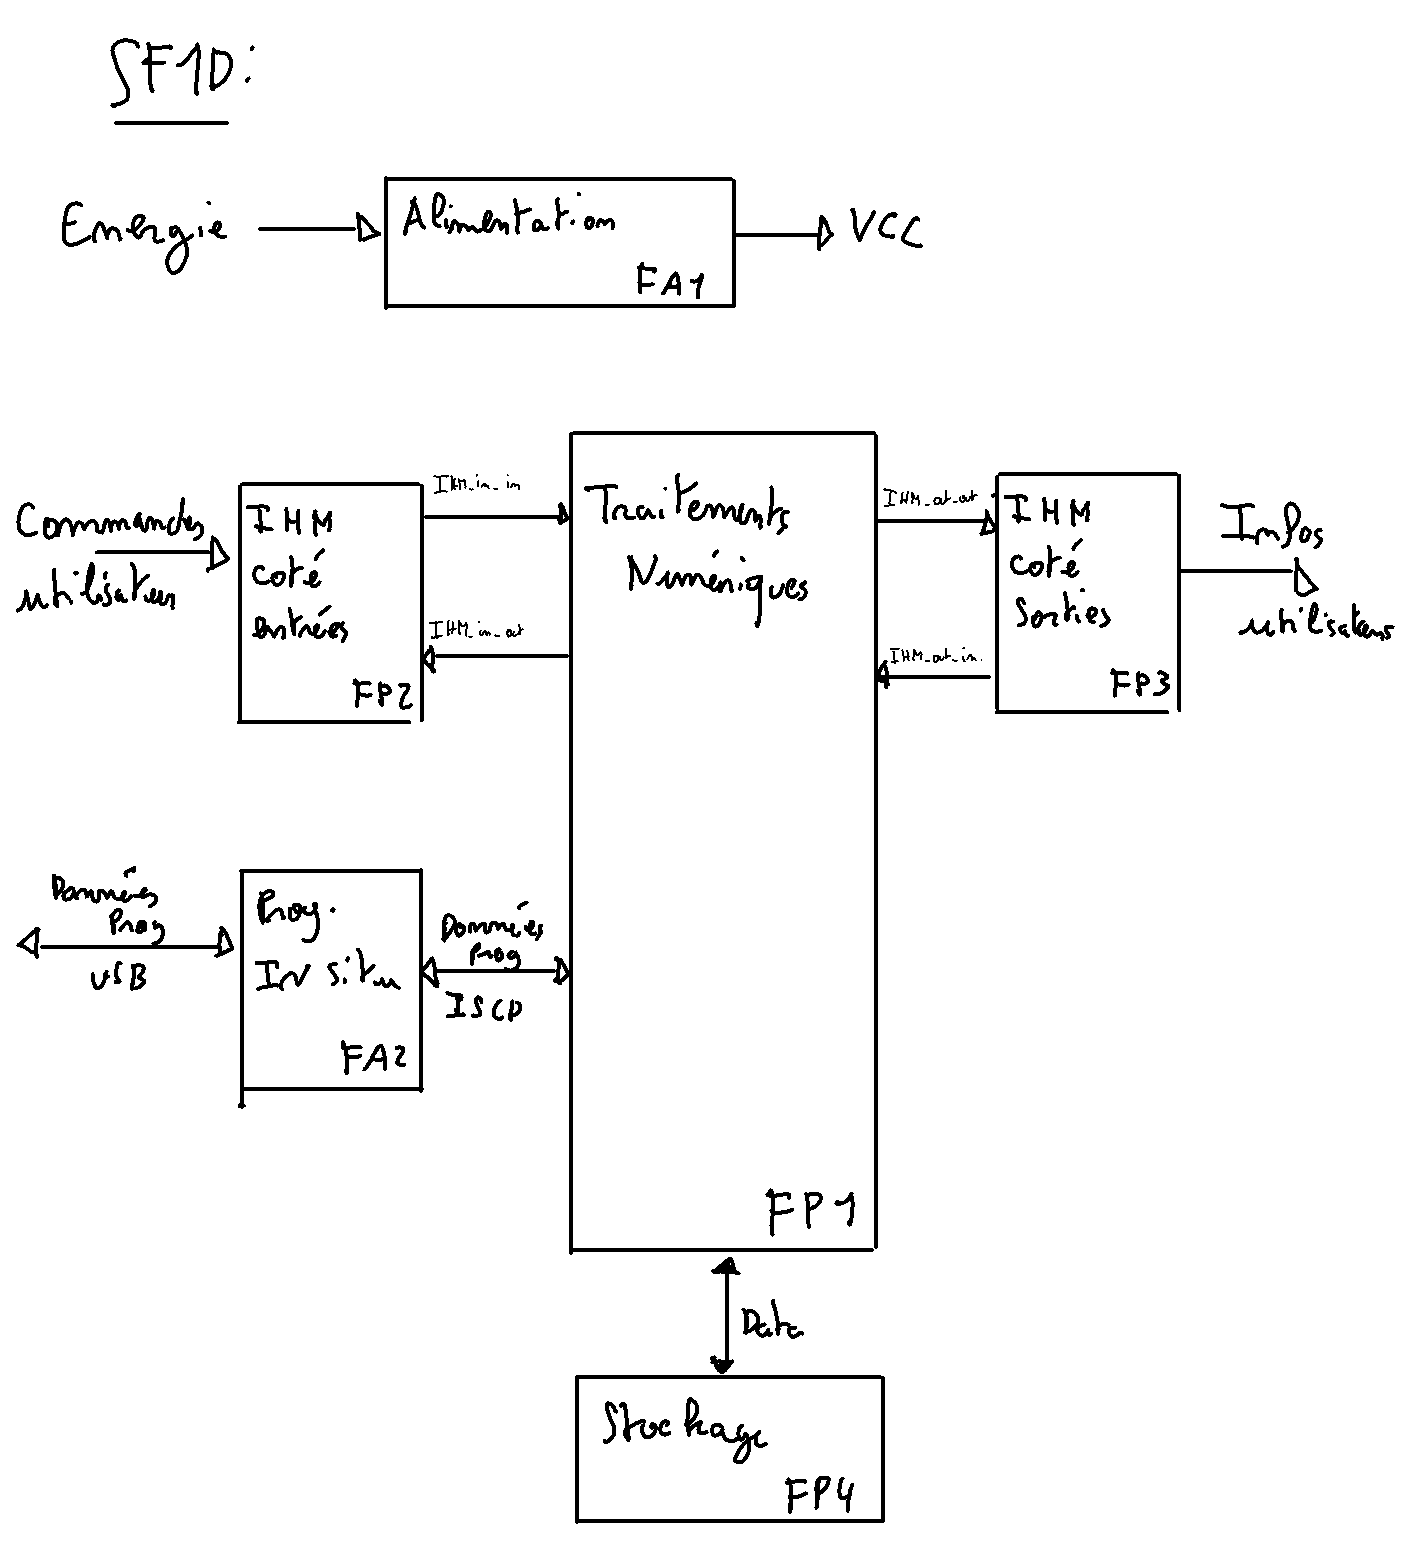
\includegraphics[width=\textwidth]{img/SF1D}
	On voit qu'on a quatre fonctions principales : une qui s'occupe de la gestion des entrées (FP2), une qui gère les sorties (FP3), une fonction de stockage pour stocker les tables de transitions (FP4), et du traitement numérique qui va piloter tout ça (FP1).\\
	On a aussi deux fonctions annexes : la fonction alimentation qui va se charger de fournir le courant nécessaire pour que la machine puisse fonctionner, et la fonction de programmation in-situ qui va faciliter le chargement du code dans la machine et nous éviter d'avoir à sortir le micro-contrôleur (MCU) à chaque fois.\\
	\\
	On voit que les fonctions FP2 et FP3 sont encore floues, on va donc les affiner en faisant des SF2D pour qu'on se rende compte de leur fonctionnement :\\
	\subsubsection{FP2 :}
	\includegraphics[width=\textwidth]{img/SF2DFP2}
	On voit clairement que FP2 est bien plus complexe qu'elle ne le parait, et forme un ensemble de fonctions plus spécifiques qui vont permettre à l'utilisateur d'interagir physiquement avec la machine, dans le but de la configurer, programmer, etc.
	\subsubsection{FP3 :}
	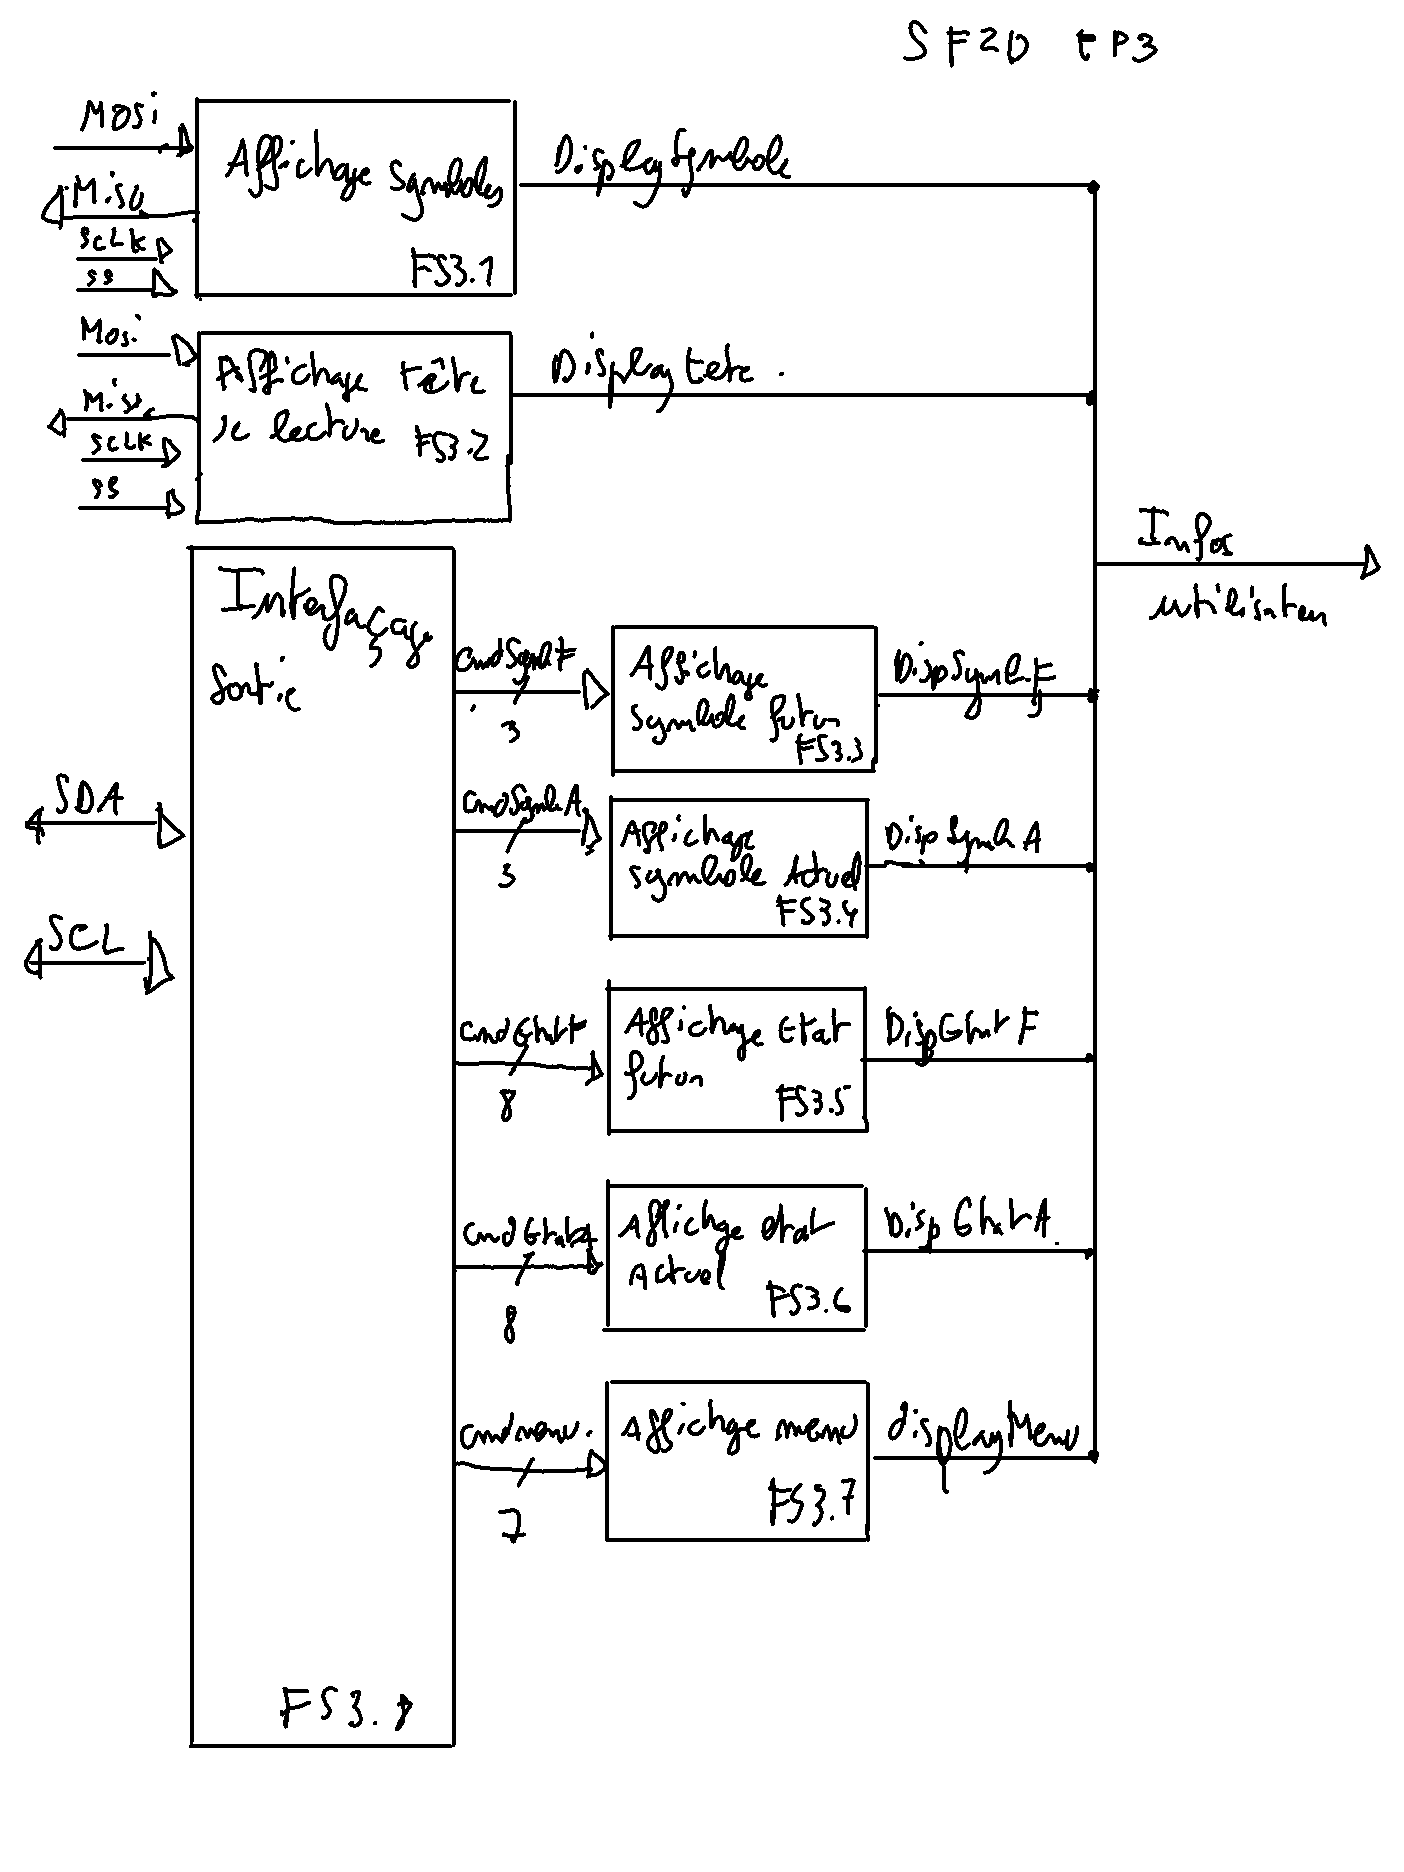
\includegraphics[width=\textwidth]{img/SF2DFP3}
	De la même manière que pour FP2, FP3 est en réalité un ensemble de fonctions plus spécifiques qui vont chacune avoir un rôle bien précis dans le retour des informations utilisateur. On a donc une grande variété de fonctions d'affichage qui vont, de la même manière que pour les sous-fonctions de FP2, être spécifiées ci-dessous.
	\subsection{Choix des technologies}
	\subsubsection{Communication}
	\paragraph{Bus I²C}
	Le nombre élevé d'entrées-sorties, du aux grand nombre de boutons poussoirs et composants d'affichage, nous a orienté sur l'utilisation d'expandeurs. Nous nous sommes orientés vers des expandeurs I²C, car l'utilisation du bus I²C nous permettait de gérer toutes nos entrées / sorties en utilisant uniquement deux broches sur le MCU (SDL et SCL). Nous avons ainsi essayé d'avoir un maximum de composants en I²C.\\
	\paragraph{Bus SPI}
	Nous nous sommes posés la question de l'utilisation du bus SPI pour notre ruban de LEDs. Nous avions aussi besoin de choisir notre type de communication avec la carte SD, et il se trouve que le bus SPI est très utilisé pour ce type de communication.\\
	\subsection{Spécifications des fonctions et de leurs signaux de communication}
	Nous avons donc spécifié ci-dessous, pour chaque fonction, son rôle ainsi que ses signaux d'entrée et/ou de sortie. Nous avons également précisé le rôle ainsi que ce qui fait l'essence même de chaque signal (type, etc.).\\
	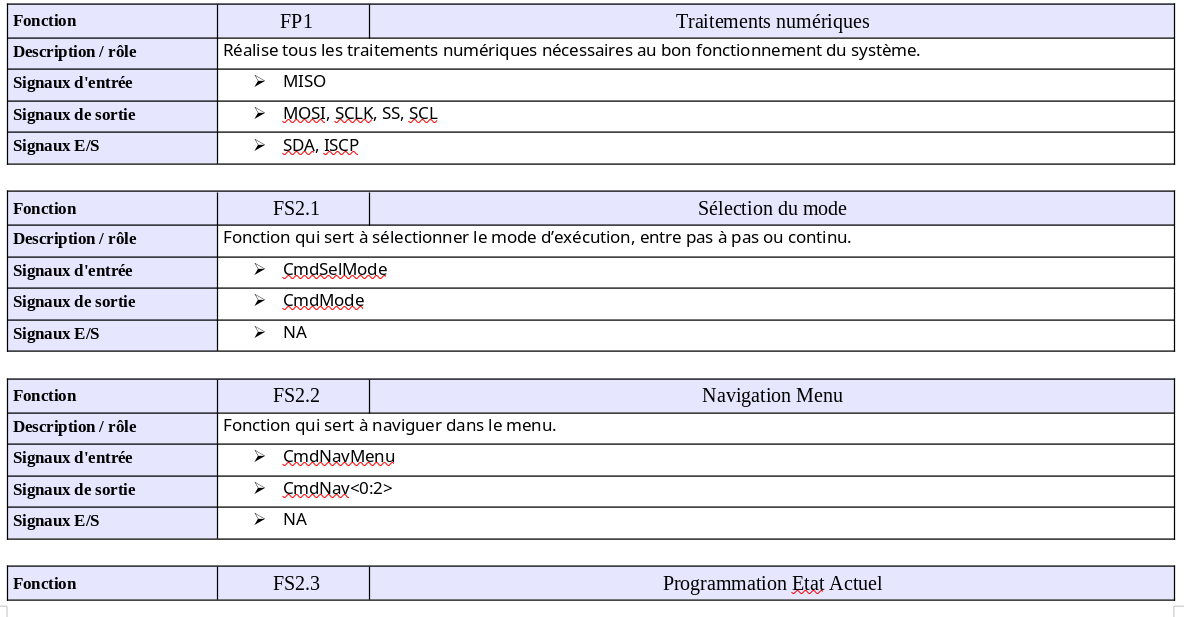
\includegraphics[width=\textwidth]{img/f1}
	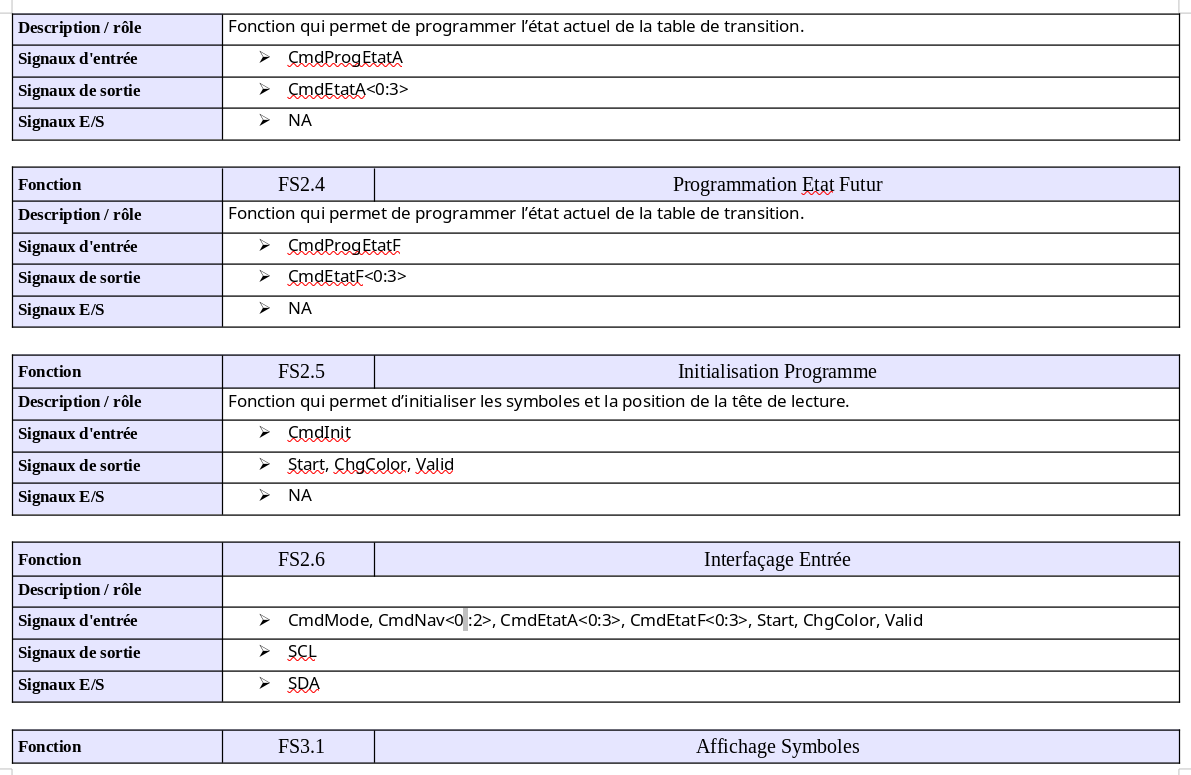
\includegraphics[width=\textwidth]{img/f2}
	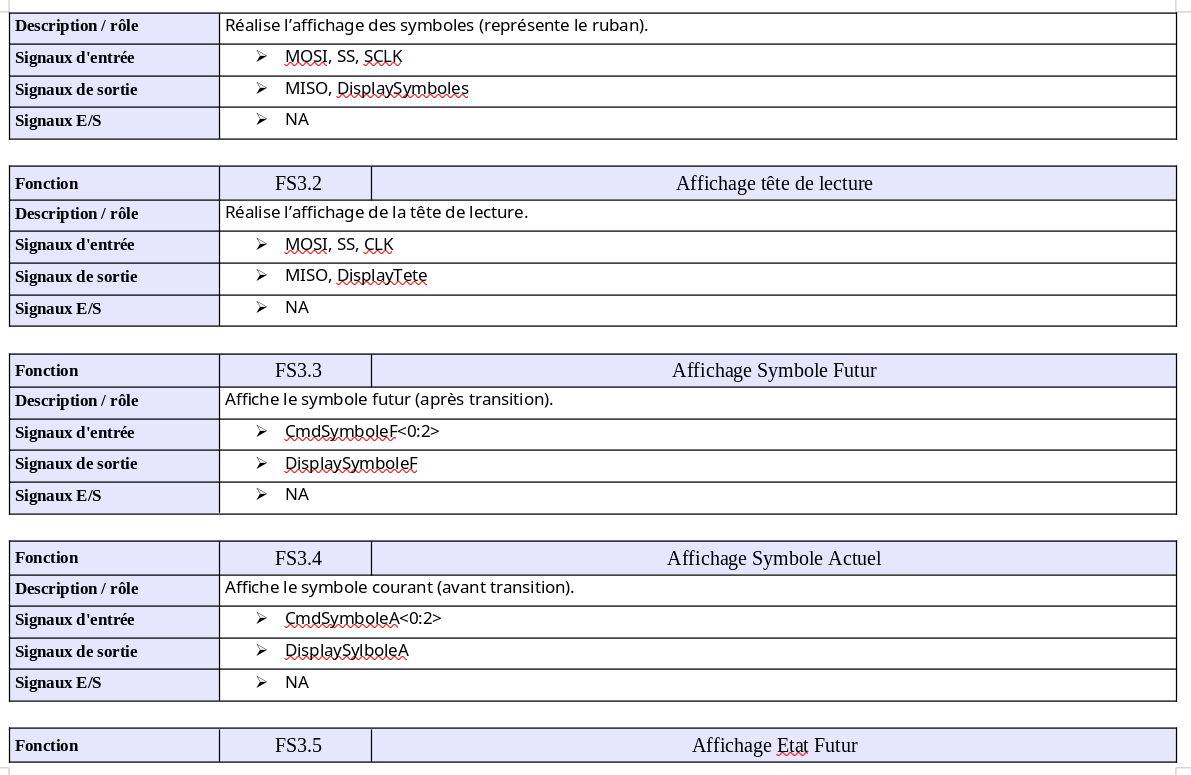
\includegraphics[width=\textwidth]{img/f3}
	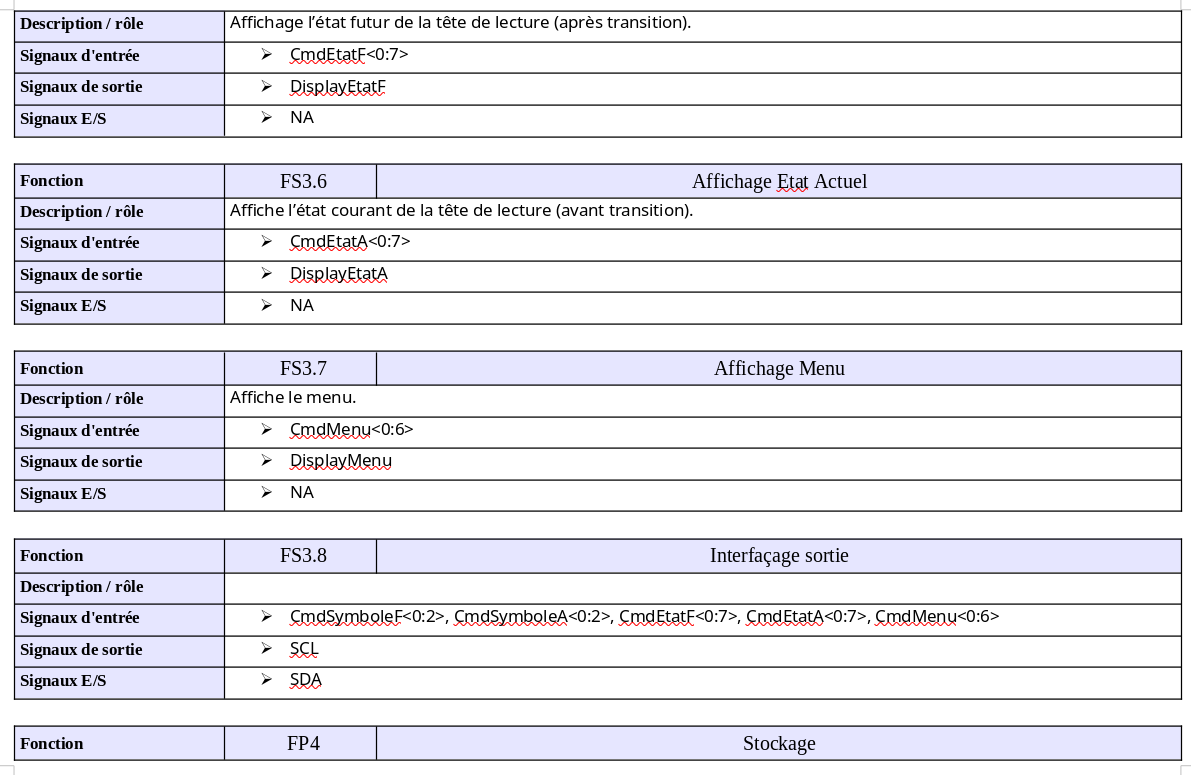
\includegraphics[width=\textwidth]{img/f4}
	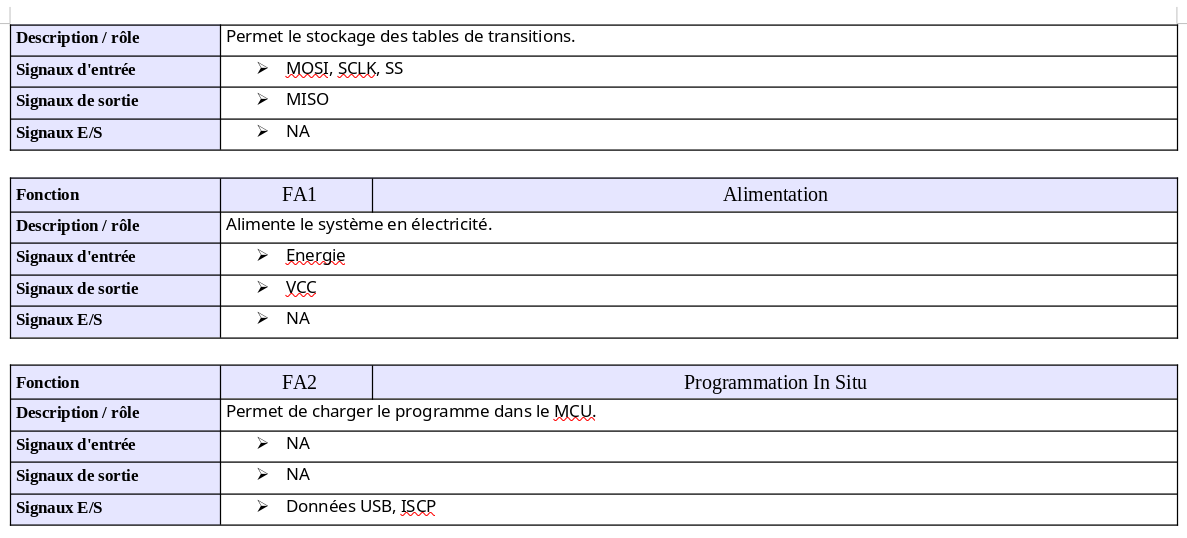
\includegraphics[width=\textwidth]{img/f5}
	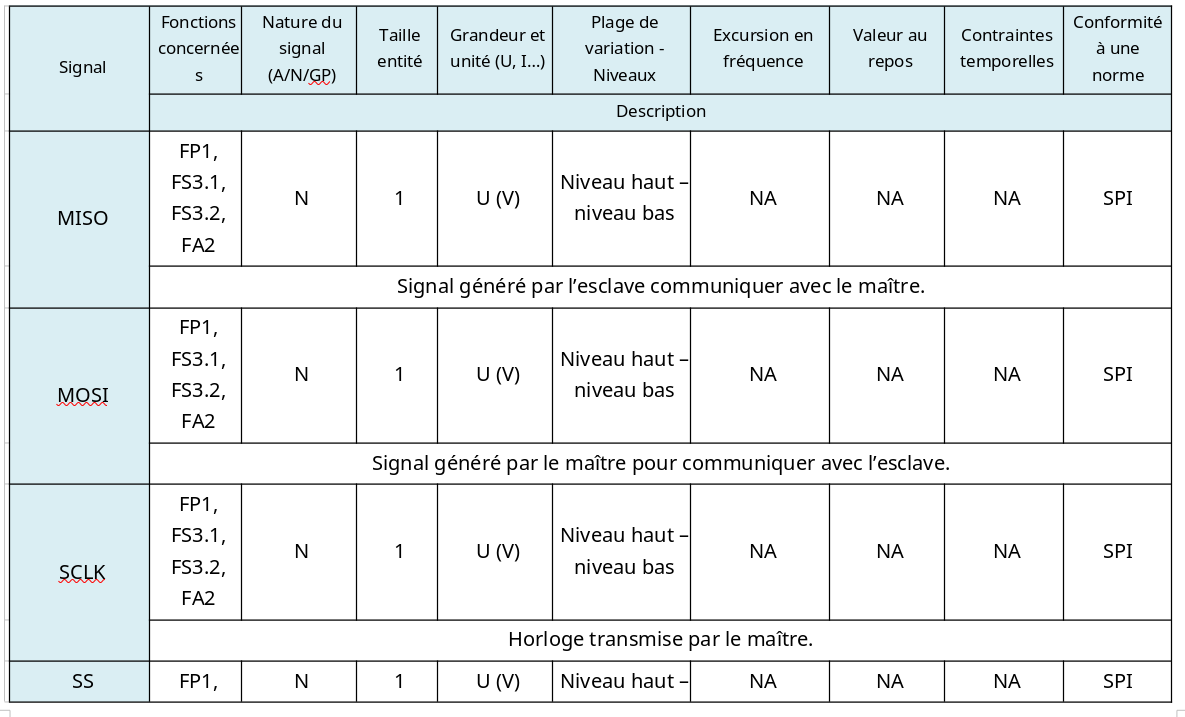
\includegraphics[width=\textwidth]{img/s1}
	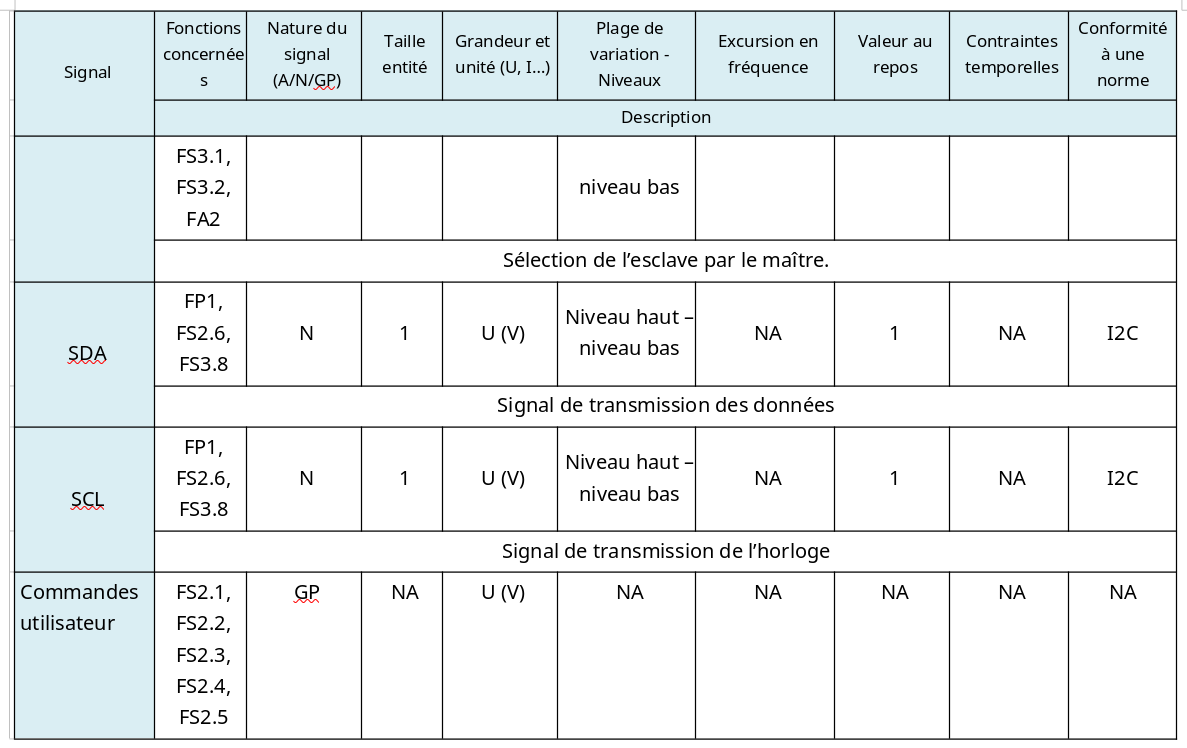
\includegraphics[width=\textwidth]{img/s2}
	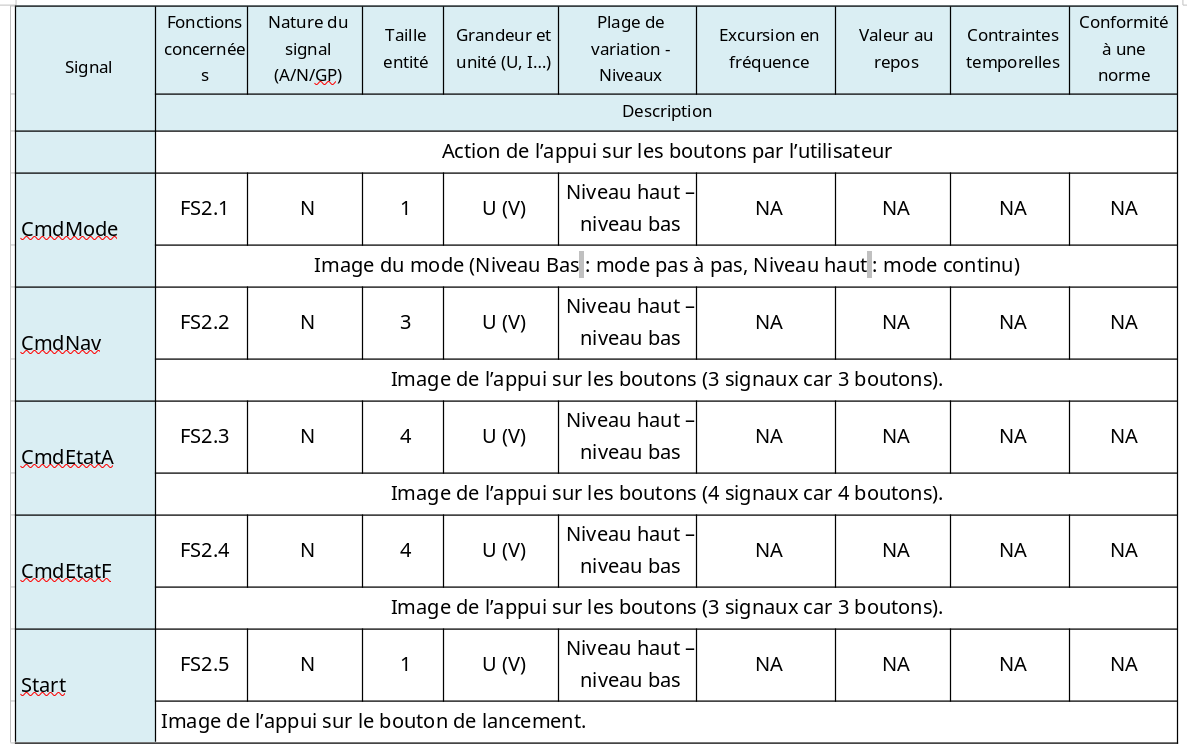
\includegraphics[width=\textwidth]{img/s3}
	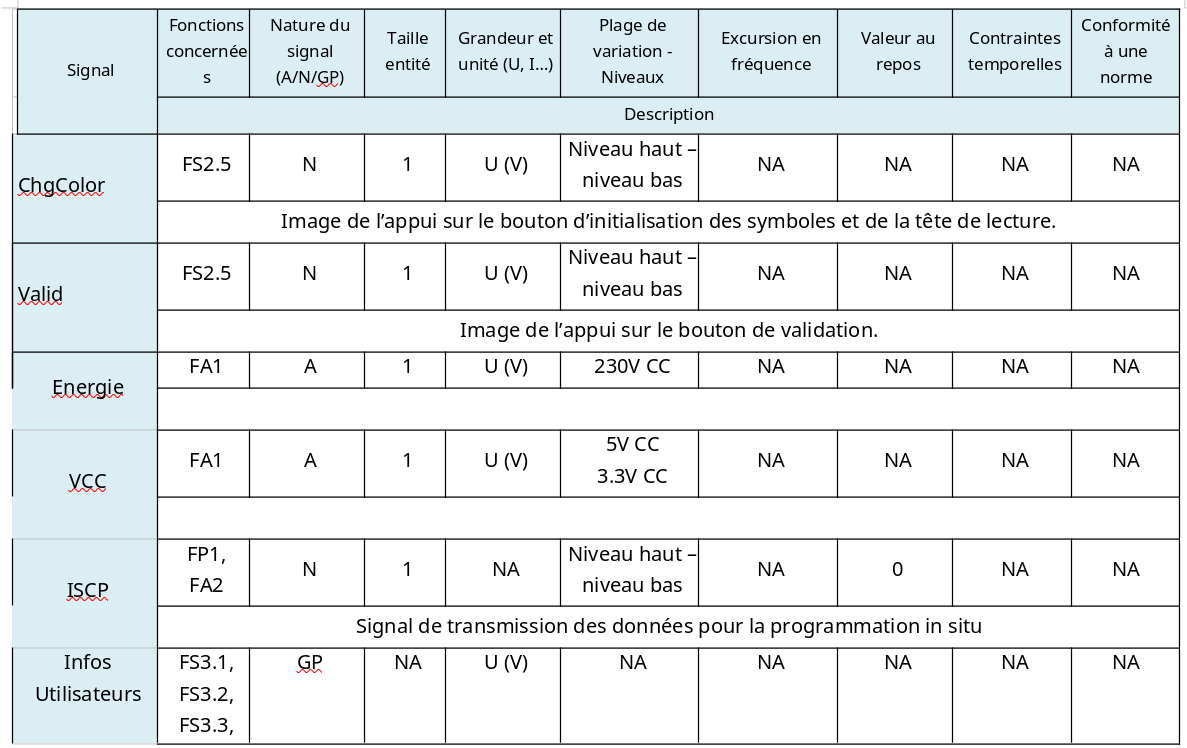
\includegraphics[width=\textwidth]{img/s4}
	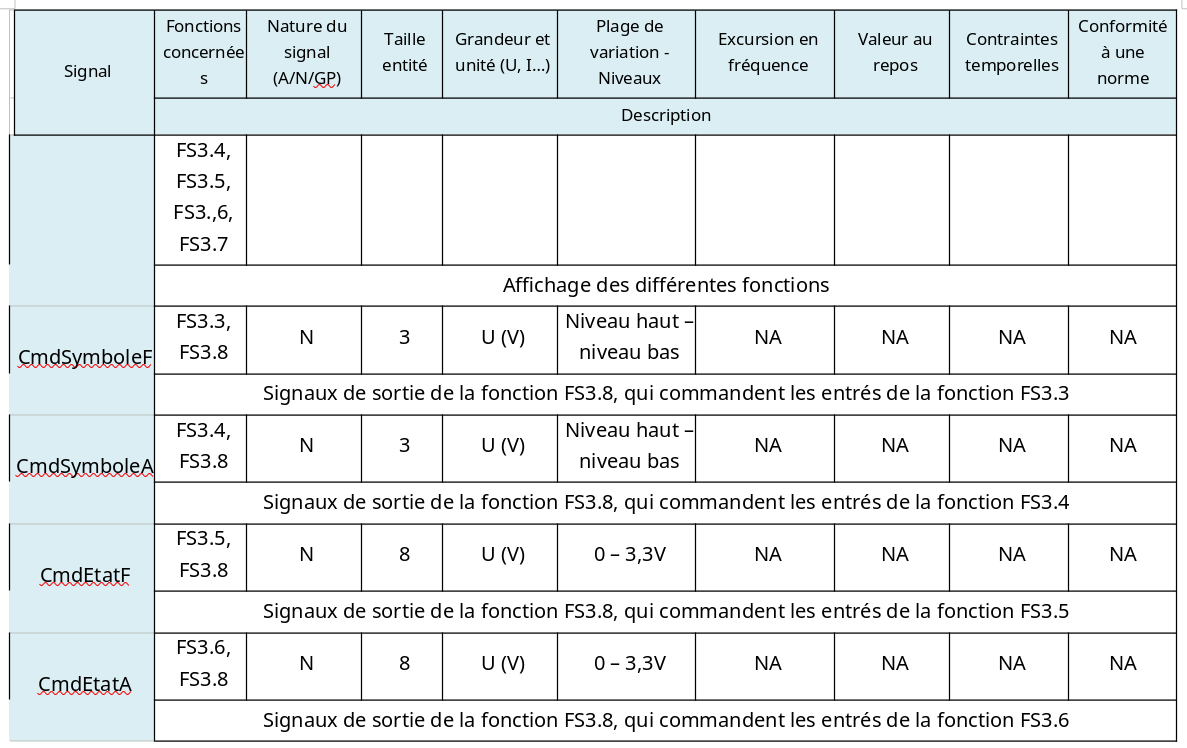
\includegraphics[width=\textwidth]{img/s5}
	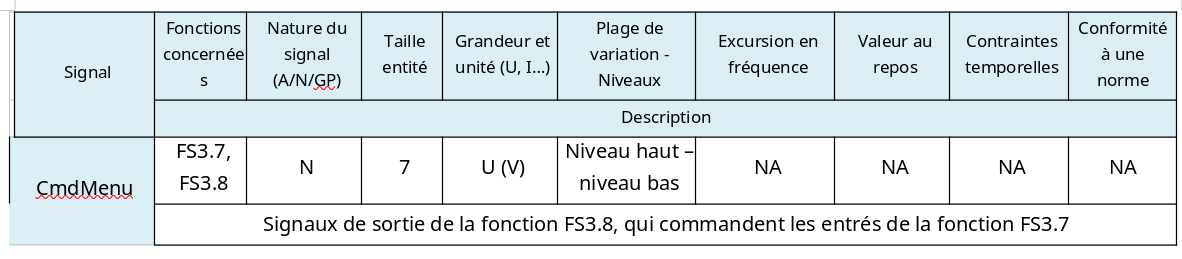
\includegraphics[width=\textwidth]{img/s6}
	\subsection{Choix des composants}
	\subsubsection{Composants}
	Nous avions donc besoin des composants suivants :
	\begin{itemize}[label=$-$]
		\item 2 rubans de LEDs RGB communicant en SPI
		\item 2 afficheurs 7 segments
		\item 1 écran LCD communicant en I²C
		\item 2 LEDs RBG
		\item 2 LEDs pour indiquer le mouvement, et 1 LED d'erreur
		\item 15 boutons poussoirs
		\item 2 commutateurs à bascule
		\item 1 lecteur de carte micro-SD communicant en SPI
		\item 3 expandeurs E/S - I²C de 16 I/O
	\end{itemize}
	\subsubsection{Choix du micro contrôleur}
	Nous avions déjà un PIC24FJ64GA002 car c'est le micro-contrôleur que le groupe précédent utilisait. Ce micro-contrôleur s'alimente en 3,3V et possède deux modules I²C et deux modules SPI. Comme nous utilisons des expandeurs pour toutes nous E/S, nous pouvons reprendre ce micro-contrôleur pour notre machine de Turing.\\
	\subsubsection{Commandes}
	Initialement, nous avions fait un premier choix de composants qui correspondait à nos spécificités. Tous les composants s'alimentent en 3,3 ou 5V. Toute la commande était prévue chez Farnell, mais nous avons dû nous raviser et mettre au point une autre liste à cause du délai de commande trop important.\\
	\paragraph{Commande initiale Farnell}
	\begin{itemize}[label=$-$]
		\item rubans de LEDs adressables \href{https://fr.aliexpress.com/item/1005006918408592.html?spm=a2g0o.productlist.main.19.fbb0788296kxRo&algo_pvid=72d2c9a9-ec47-4e4b-9d14-7e90be35485c&algo_exp_id=72d2c9a9-ec47-4e4b-9d14-7e90be35485c-9&pdp_npi=4%40dis!EUR!18.92!18.92!!!145.68!145.68!%402103888a17169934968957029e0b2f!12000038723750387!sea!FR!0!AB&curPageLogUid=lAauznpLAY1Y&utparam-url=scene%3Asearch%7Cquery_from%3A}{SK9822}
		\item afficheurs 7 segments \href{https://fr.farnell.com/broadcom-limited/hdsm-283b/afficheur-a-led-cms-7mm-bleu-cc/dp/1659312}{HDSM-283B}
		\item LEDs RGB \href{https://fr.farnell.com/kingbright/l-59eyc/led-5mm-tricolore/dp/1168662}{L-59EYC}
		\item expandeurs E/S - I²C \href{https://fr.farnell.com/microchip/mcp23017-e-sp/16-bit-expander-i-o-i2c-i-f/dp/1332088}{MCP23017}
		\item écran LCD I2C \href{https://fr.farnell.com/midas/mc21605c6w-bnmlwi-v2/afficheur-alphanumerique-16x2/dp/2748649}{MC21605C6W-BNMLWI-V2}
		\item boutons poussoirs \href{https://fr.farnell.com/panasonic/ese20c321/commutateur-bouton-pouss-momentane/dp/2079613}{ESE20C321}
		\item commutateurs \href{https://fr.farnell.com/multicomp/2as2t2a1m7re/switch-toggle-spdt-on-mom/dp/1550118}{2AS2T2A1M7RE}
	\end{itemize}
	\paragraph{Commande réelle (RS et Amazon)}
	\begin{itemize}[label=$-$]
		\item rubans de LEDs adressables \href{https://fr.aliexpress.com/item/1005006918408592.html?spm=a2g0o.productlist.main.19.fbb0788296kxRo&algo_pvid=72d2c9a9-ec47-4e4b-9d14-7e90be35485c&algo_exp_id=72d2c9a9-ec47-4e4b-9d14-7e90be35485c-9&pdp_npi=4%40dis!EUR!18.92!18.92!!!145.68!145.68!%402103888a17169934968957029e0b2f!12000038723750387!sea!FR!0!AB&curPageLogUid=lAauznpLAY1Y&utparam-url=scene%3Asearch%7Cquery_from%3A}{SK9822}
		\item expandeurs E/S - I²C \href{https://fr.farnell.com/microchip/mcp23017-e-sp/16-bit-expander-i-o-i2c-i-f/dp/1332088}{MCP23017}
		\item écran LCD I²C \href{https://fr.rs-online.com/web/p/afficheurs-monochromes-lcd/2644045?searchId=b08a66da-698d-420f-a525-b4944d7ccd96&gb=s}{NHD-C0220BiZ-FSW-FBW-3V3M}\\
		\item LEDs RGB \href{https://fr.rs-online.com/web/p/leds/1651767?gb=s}{L-154A4SURKQBDZGW}
	\end{itemize}
	\subsection{Schéma représentatif}
	Le schéma ci-dessous nous donne une idée de ce à quoi pourrait ressembler notre machine de Turing une fois tous les composants montés :\\
	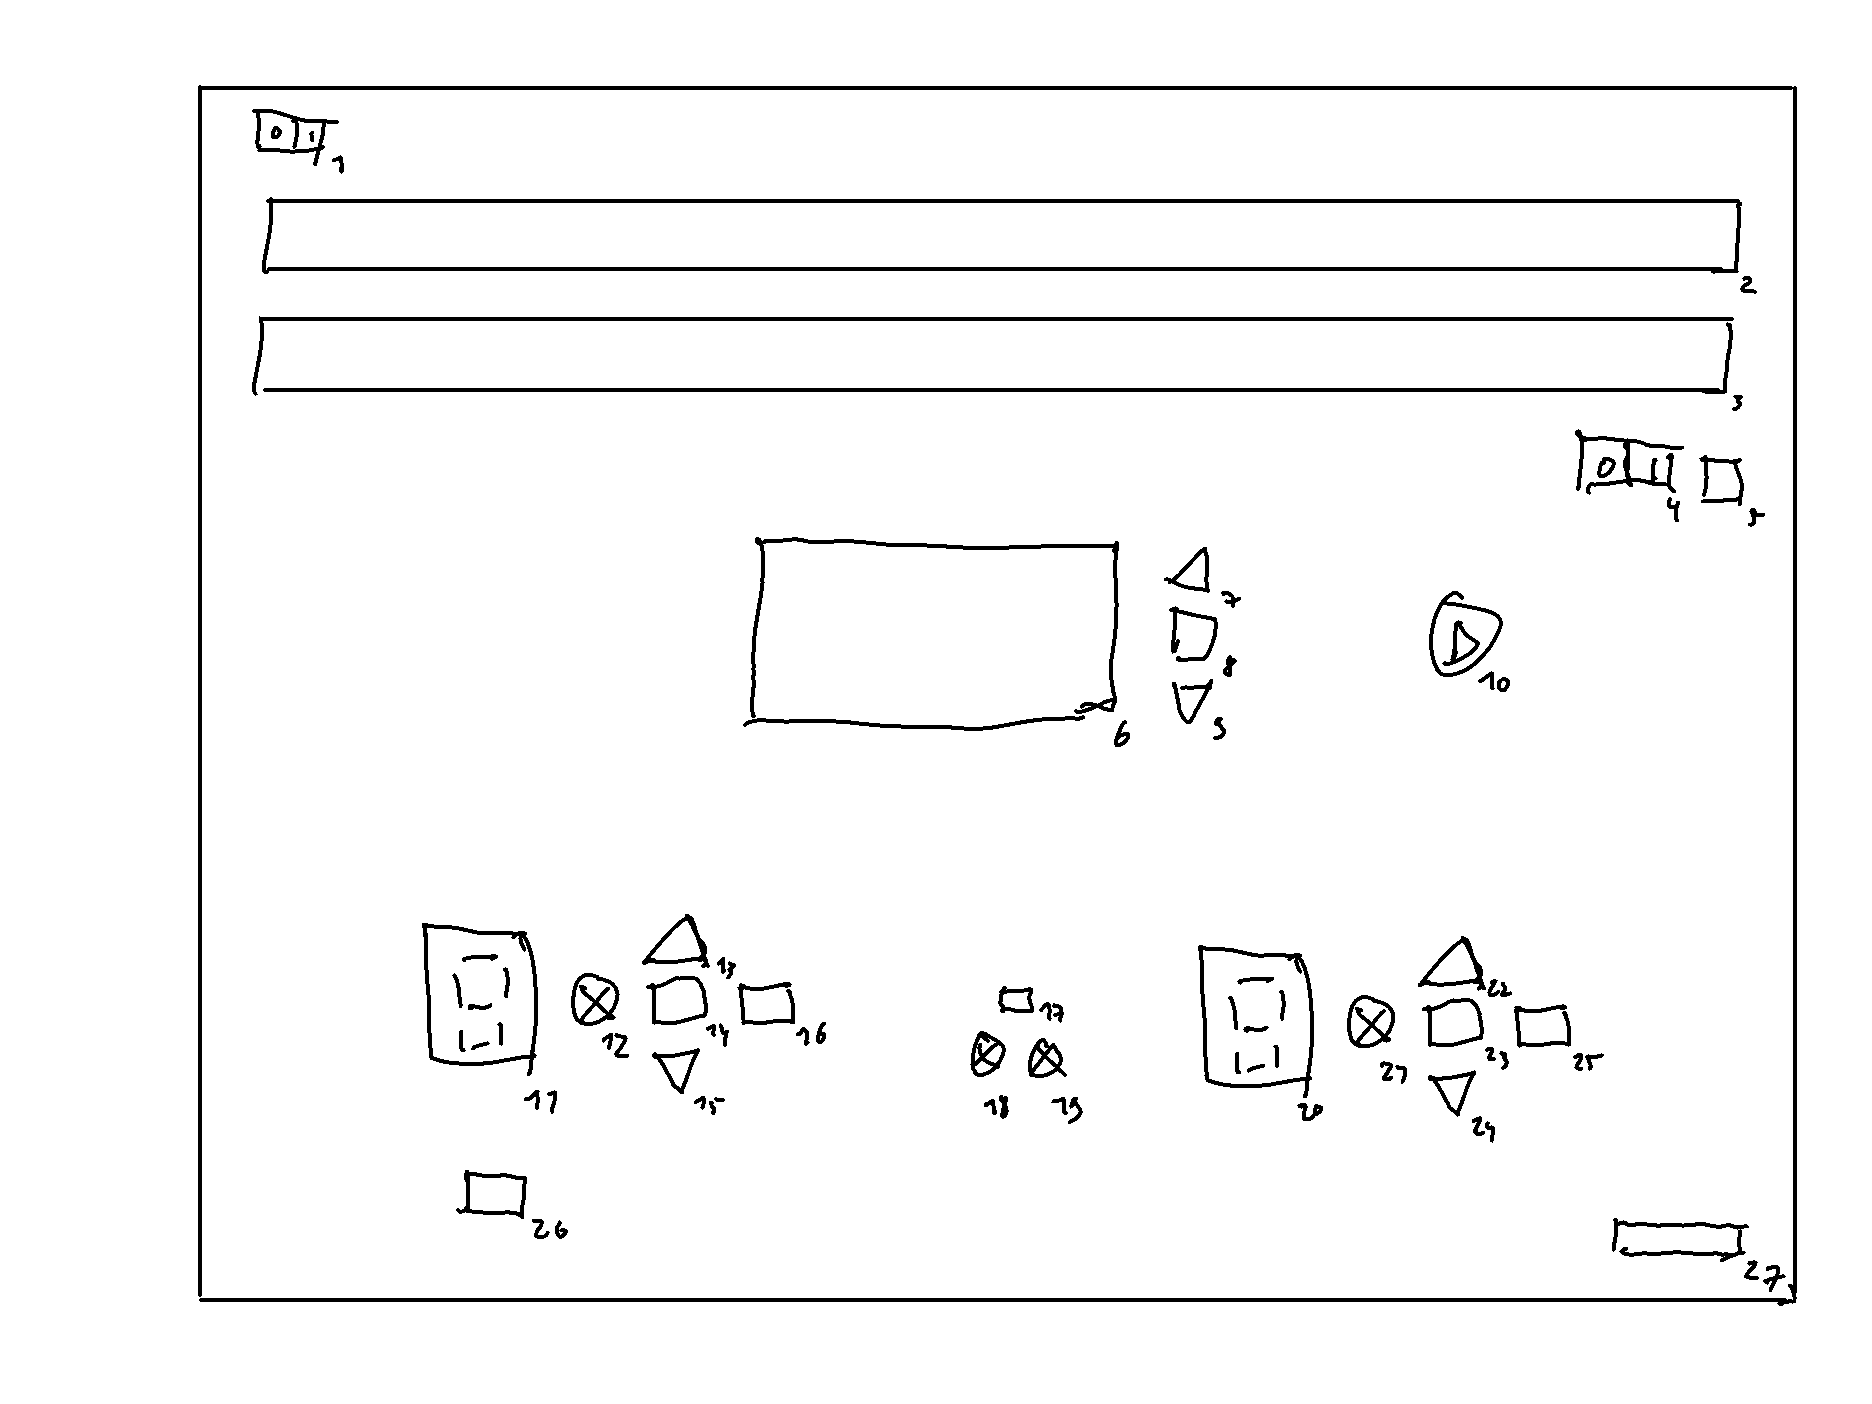
\includegraphics[width=\textwidth]{img/rep_machine}
	\\
	\\
	Nous avons essayé de respecter les connexions minimales recommandées de Microchip, trouvées dans la documentation de notre micro-contrôleur à la page 17 (voir \hyperref[sec:an4.1]{Annexe 4.1}).
	Légende :\\
	\begin{itemize}[label=$-$]
		\item 1: Interrupteur d'alimentation
		\item 2: Ruban de LEDs pour l'affichage des symboles
		\item 3: Ruban de LEDs pour l'affichage de la tête de lecture
		\item 4: Commutateur pour choisir entre le mode pas à pas et automatique
		\item 5: Bouton de réinitialisation lors de l'initialisation manuelle des rubans de LEDs
		\item 6: Ecran LCD pour l'affichage du menu
		\item 7, 8, 9: Boutons de navigation dans le menu (monter, sélectionner, descendre)
		\item 10: Bouton de lancement du programme. Sert également à passer à l'étape suivante en mode pas à pas
		\item 11 | 20: Afficheurs 7 segments pour l'affichage de l'état courant | de l'état suivant
		\item 12 | 21: LEDs RGB pour l'affichage du symbole courant | du symbole suivant
		\item 13, 14, 15, 16 | 22, 23, 24, 25: Boutons de décrémentation, validation, incrémentation, ré-initialisation de l'état et du symbole courant | de l'état et du symbole futur
		\item 17: Bouton de changement du déplacement pour l'état suivant
		\item 18, 19: LED représentant le déplacement pour l'état suivant (gauche si LED 18 allumée, droite si LED 19 allumée)
		\item 26: Bouton de sélection d'un état d'acceptation
		\item 27: Lecteur de carte micro-SD
	\end{itemize}
	\subsection{Schémas structurels}
	\subsubsection{MCU}
	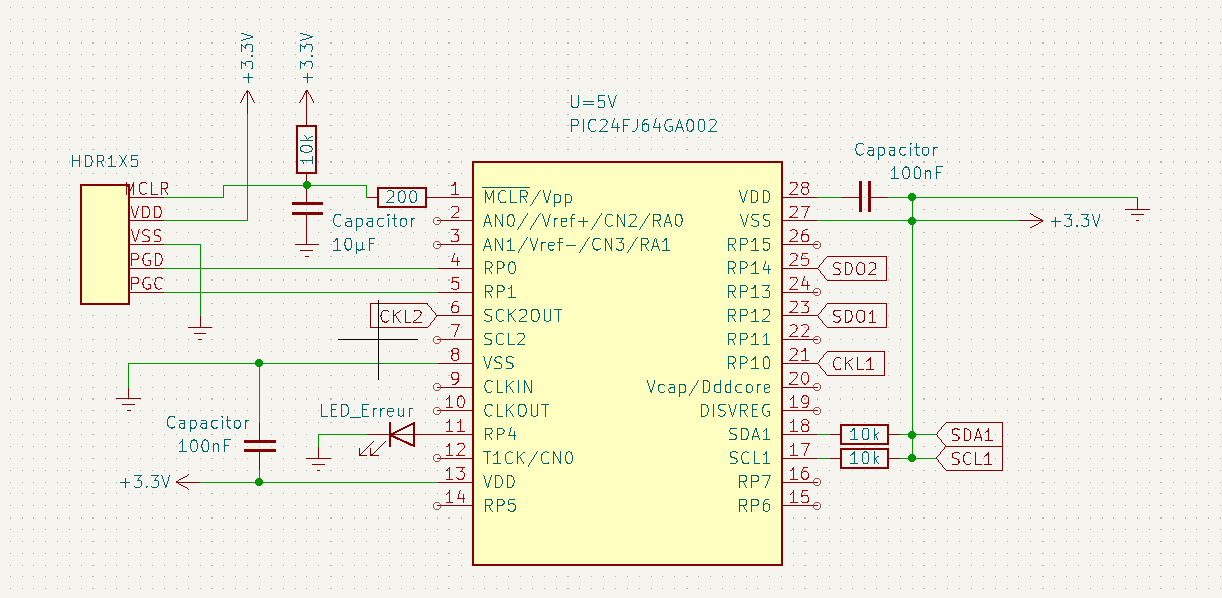
\includegraphics[width=\textwidth]{img/st_mcu}
	\subsubsection{Expandeurs E/S - I²C}
	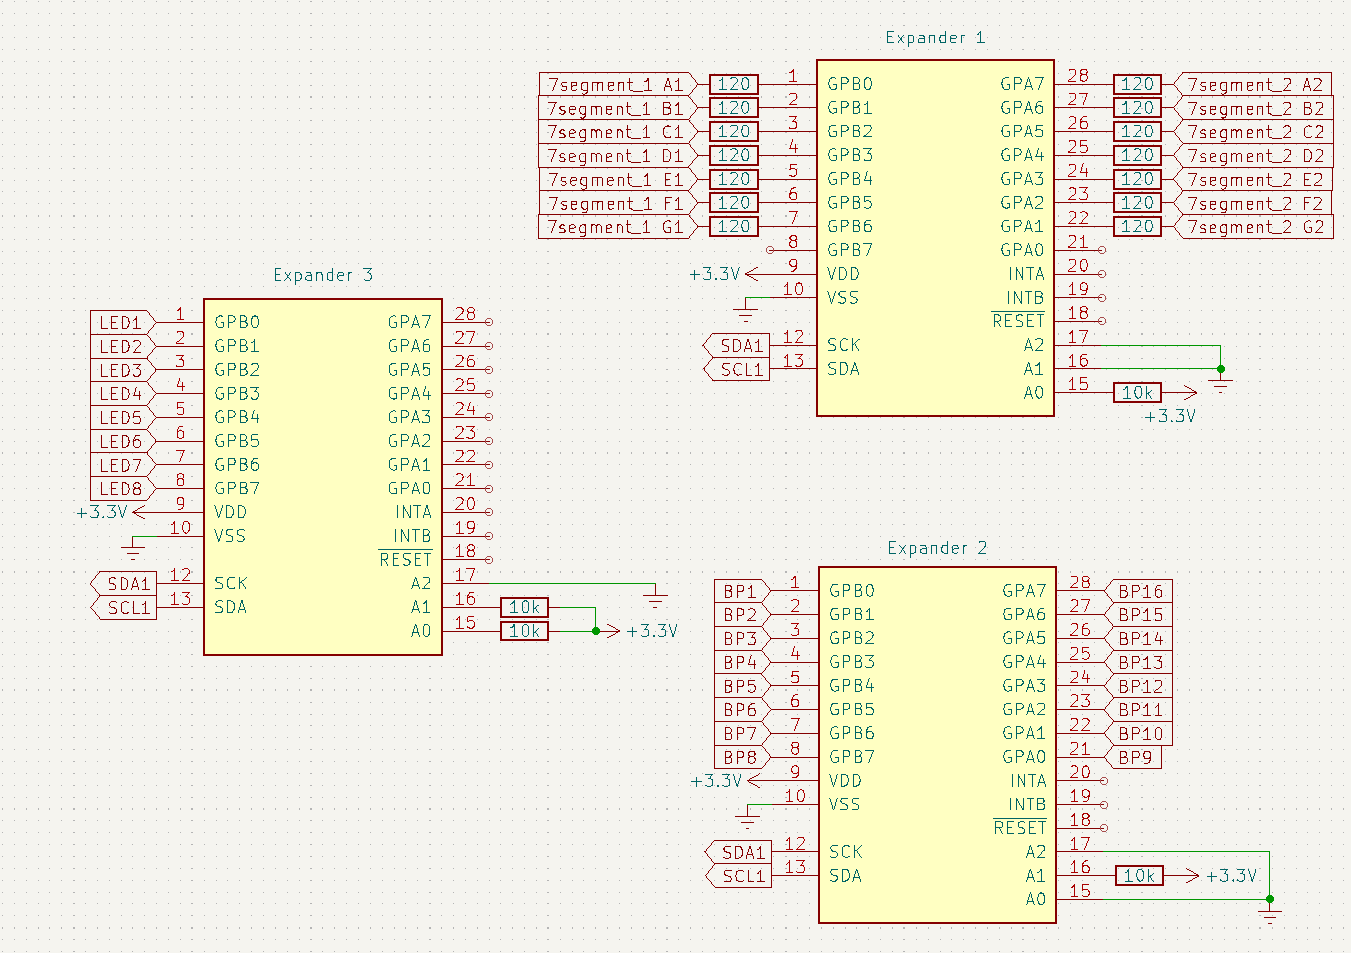
\includegraphics[width=\textwidth]{img/st_exp}
	\subsubsection{Ecran LCD}
	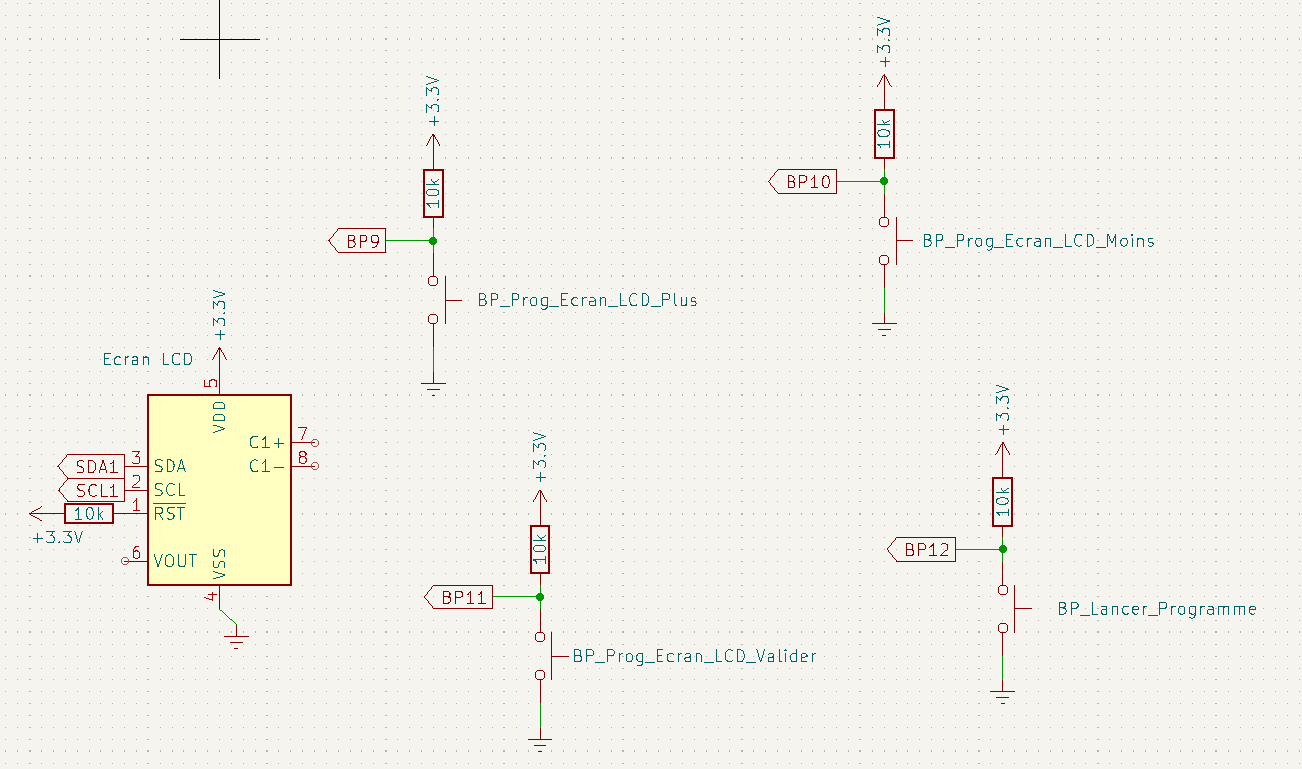
\includegraphics[width=\textwidth]{img/st_LCD}
	\subsubsection{Affichage et programmation de l'état courant}
	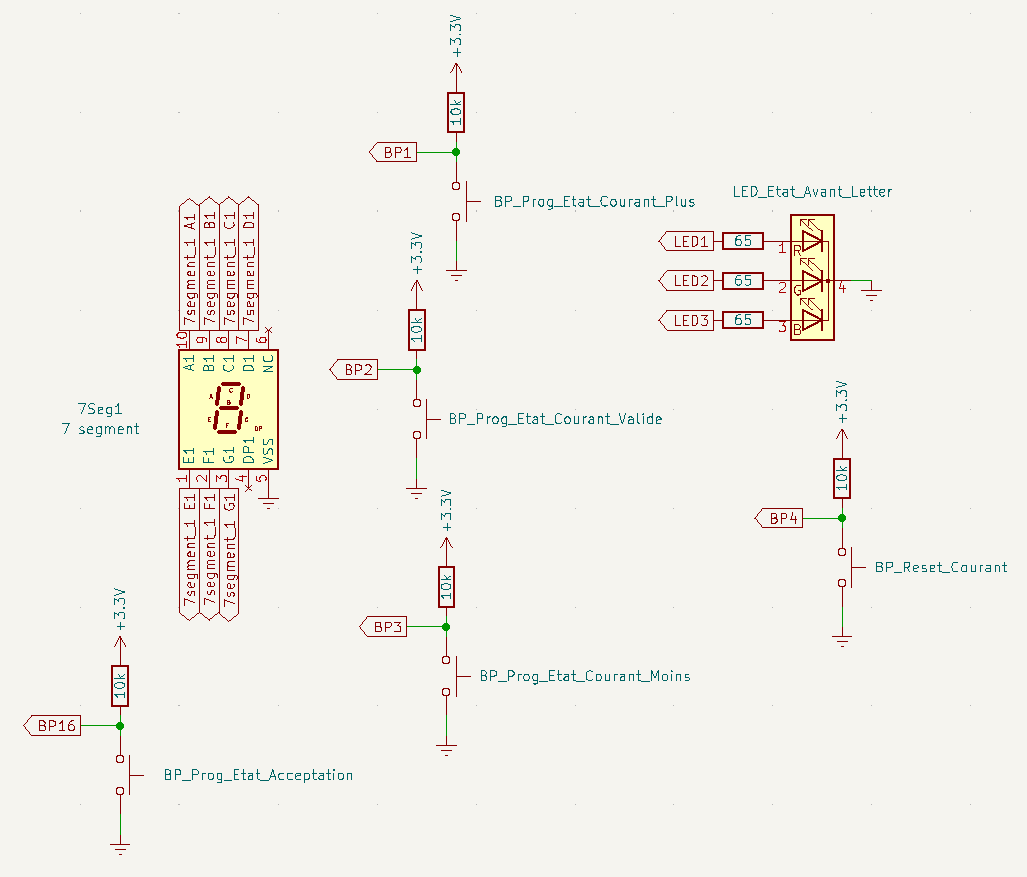
\includegraphics[width=\textwidth]{img/st_etat_courant}
	\subsubsection{Affichage et programmation de l'état futur}
	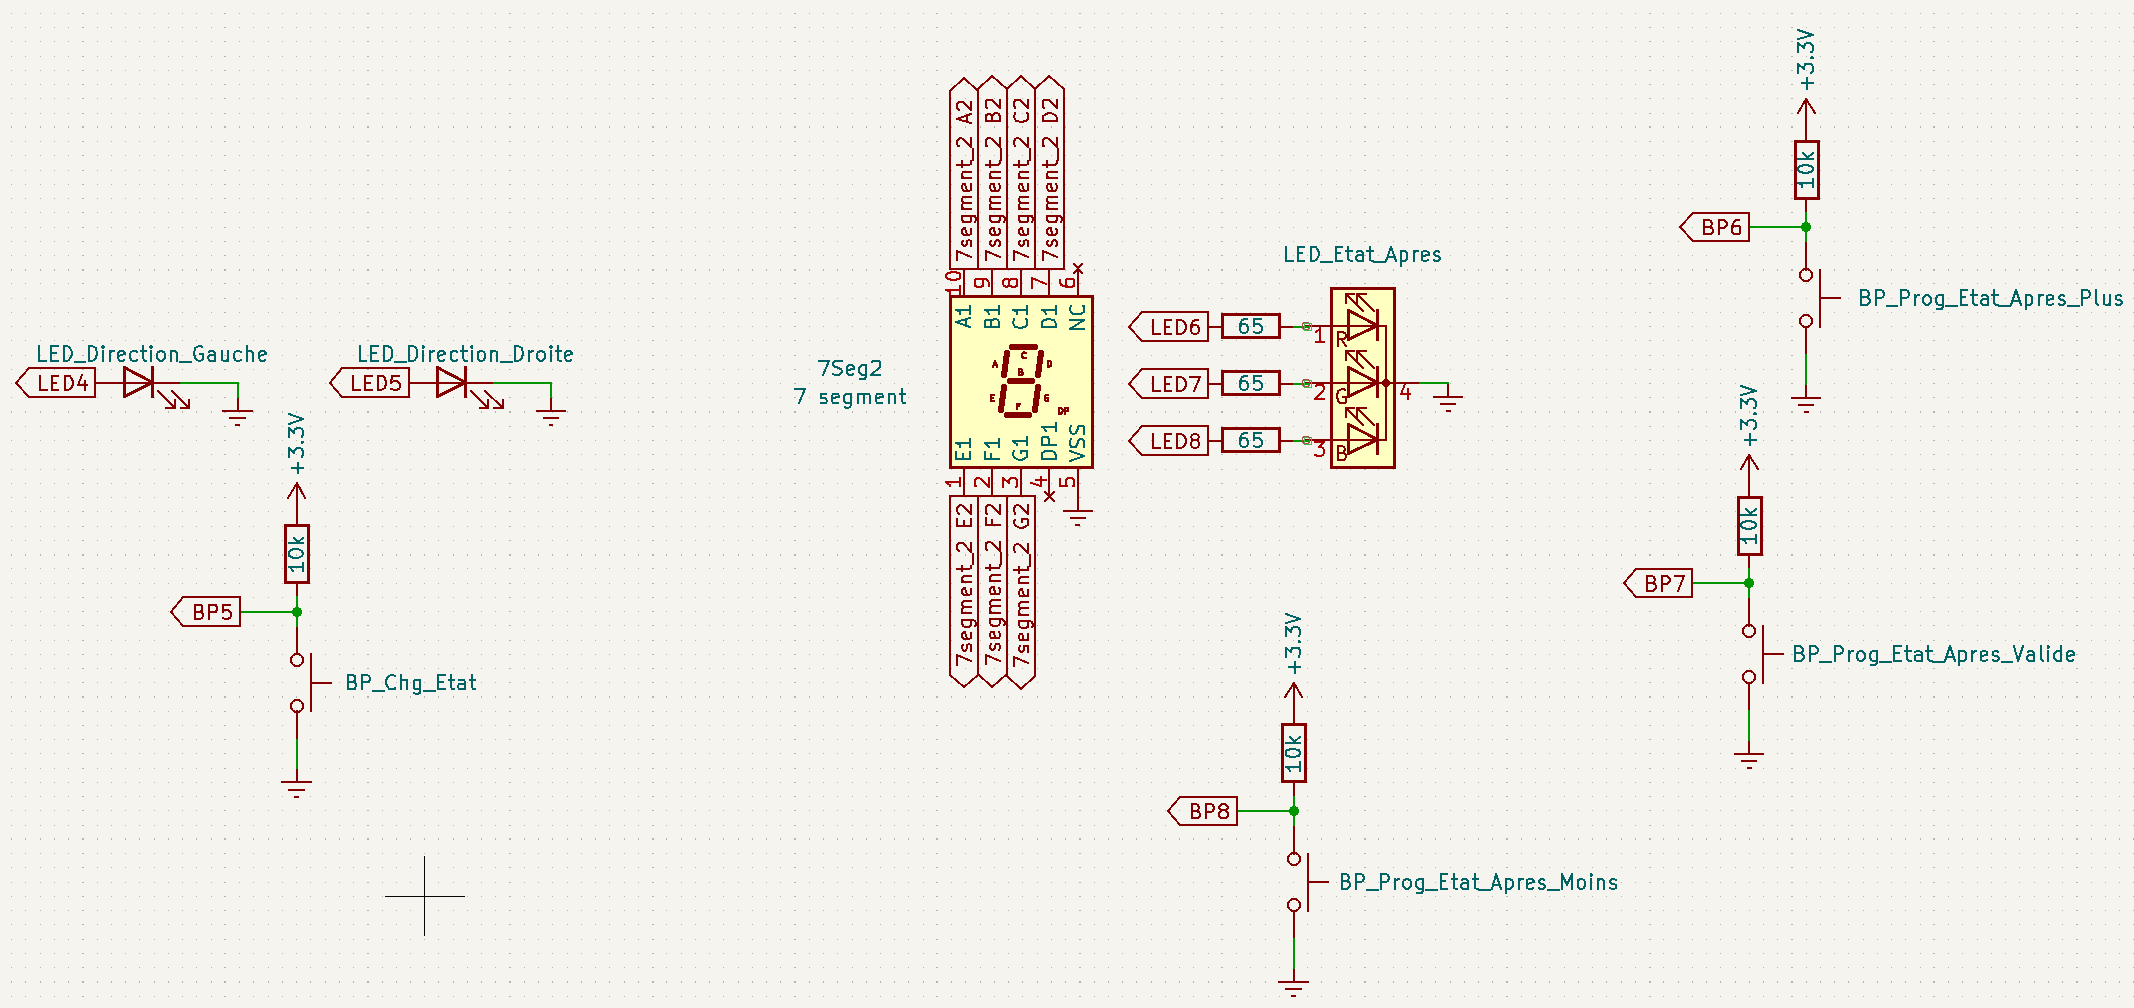
\includegraphics[width=\textwidth]{img/st_etat_futur}
	\subsection{Tests}
	Nous avons manqué de temps pour effectuer des tests. Néanmoins nous en avons écrits un, permettant de tester la communication entre le micro-contrôleur, et l'expandeur I²C :\\
	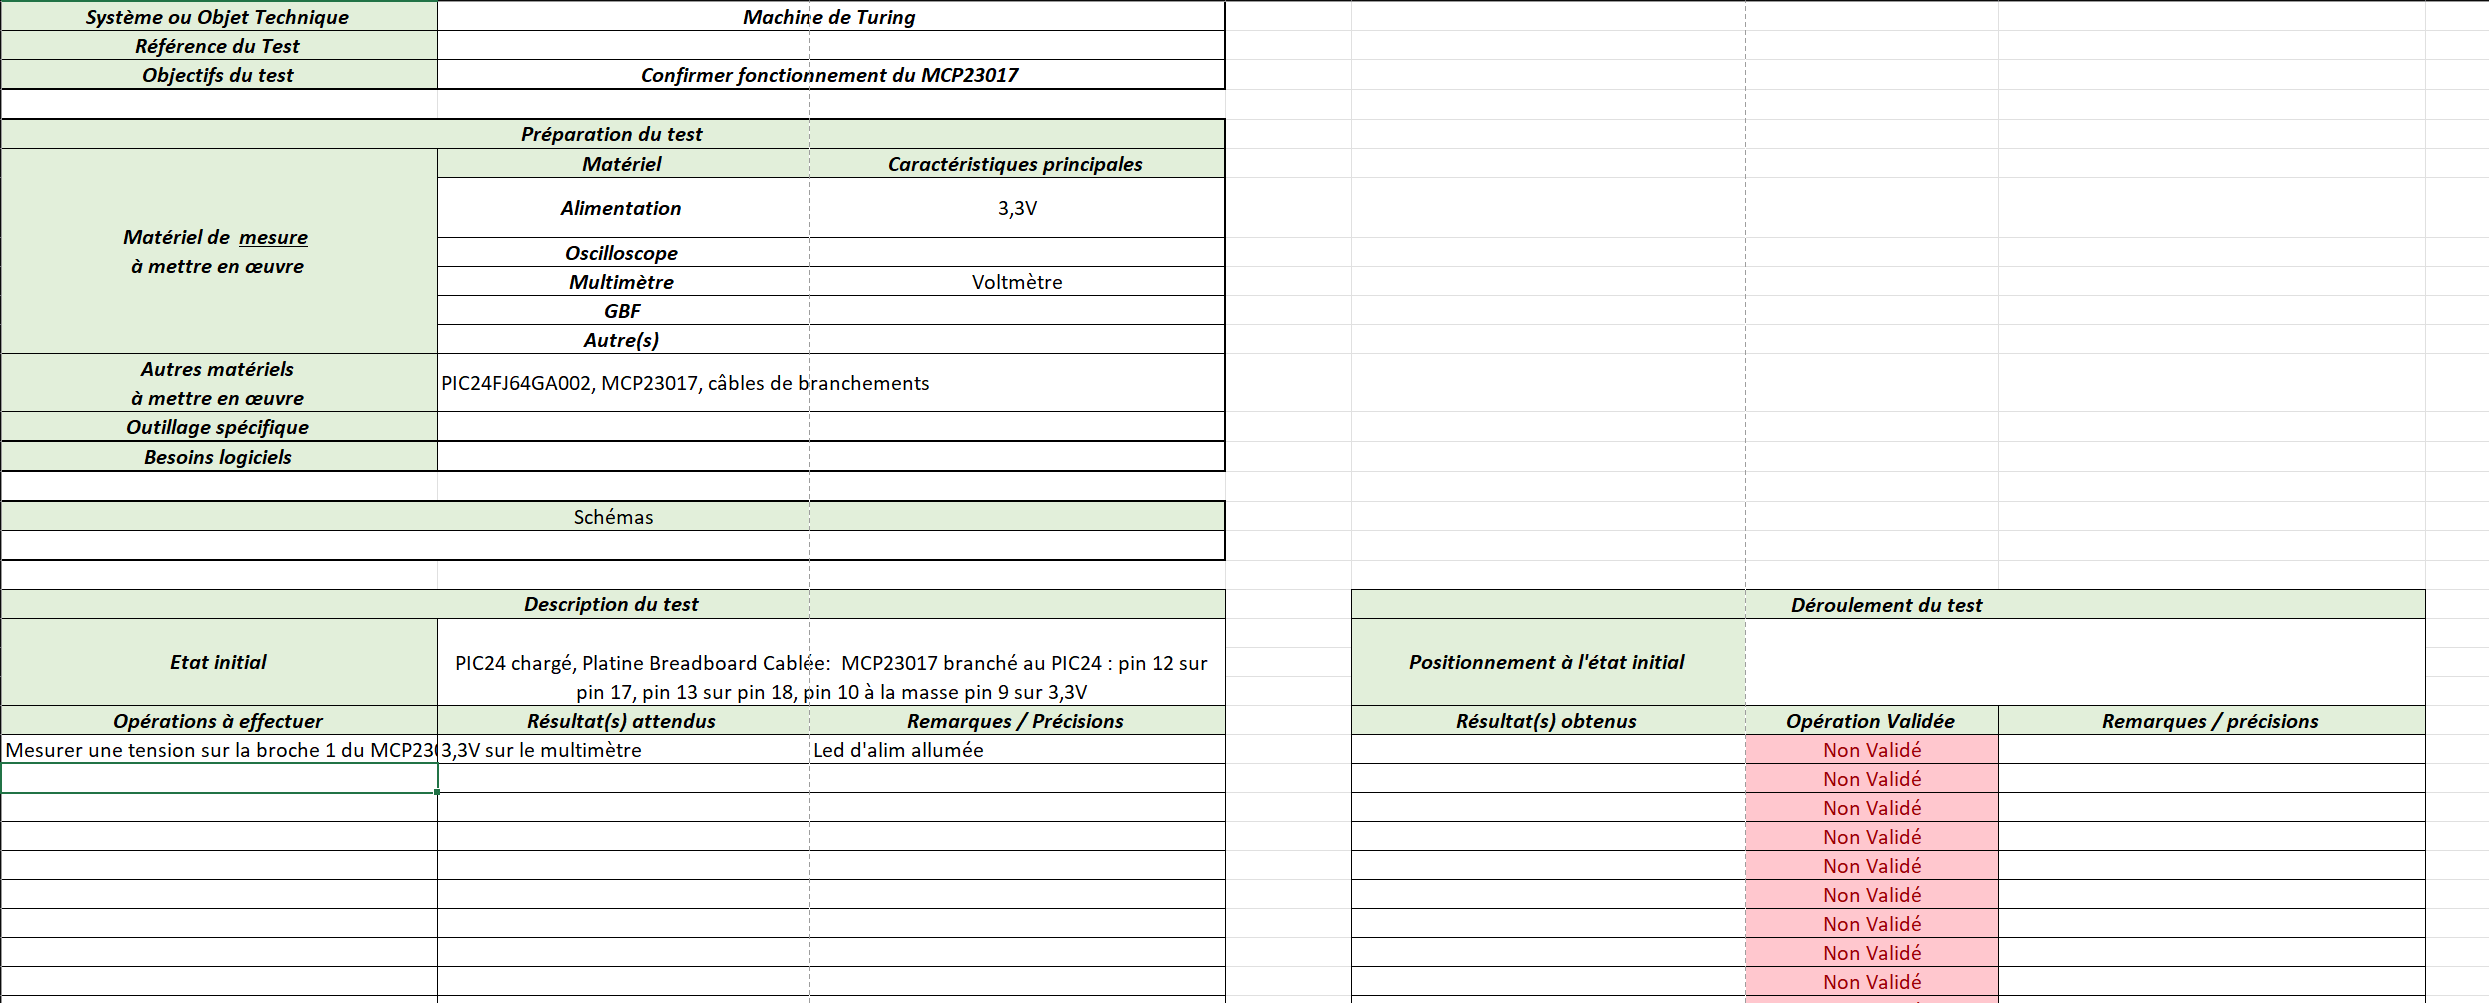
\includegraphics[width=\textwidth]{img/test}
	\subsection{Conception Logicielle}
	Cette section ne traitera que la partie 1 du cahier des charges, les parties 2 et 3 ne pouvant être réalisées par manque de temps.\\
	La table de transition "Addition de deux binaires" que nous avons utilisé pour notre machine de Turing est disponible à \hyperref[sec:an4.2]{l'annexe 4.2}
	\subsection{Diagramme de Séquences}
	Les deux diagrammes de séquence ci-dessous montrent respectivement la phase d'initialisation et la phase de déroulement du programme au niveau du micro-contrôleur (on ne prend pas en compte les actions de l'utilisateur).\\
	Ce sont des diagrammes "best-case", c'est à dire qu'on ne prend pas en compte les erreurs qui pourraient survenir, et on déroule le fonctionnement du programme en supposant que tout se passe bien. Cela permet principalement de ne pas faire trop de diagrammes, ni de diagrammes trop longs.\\
	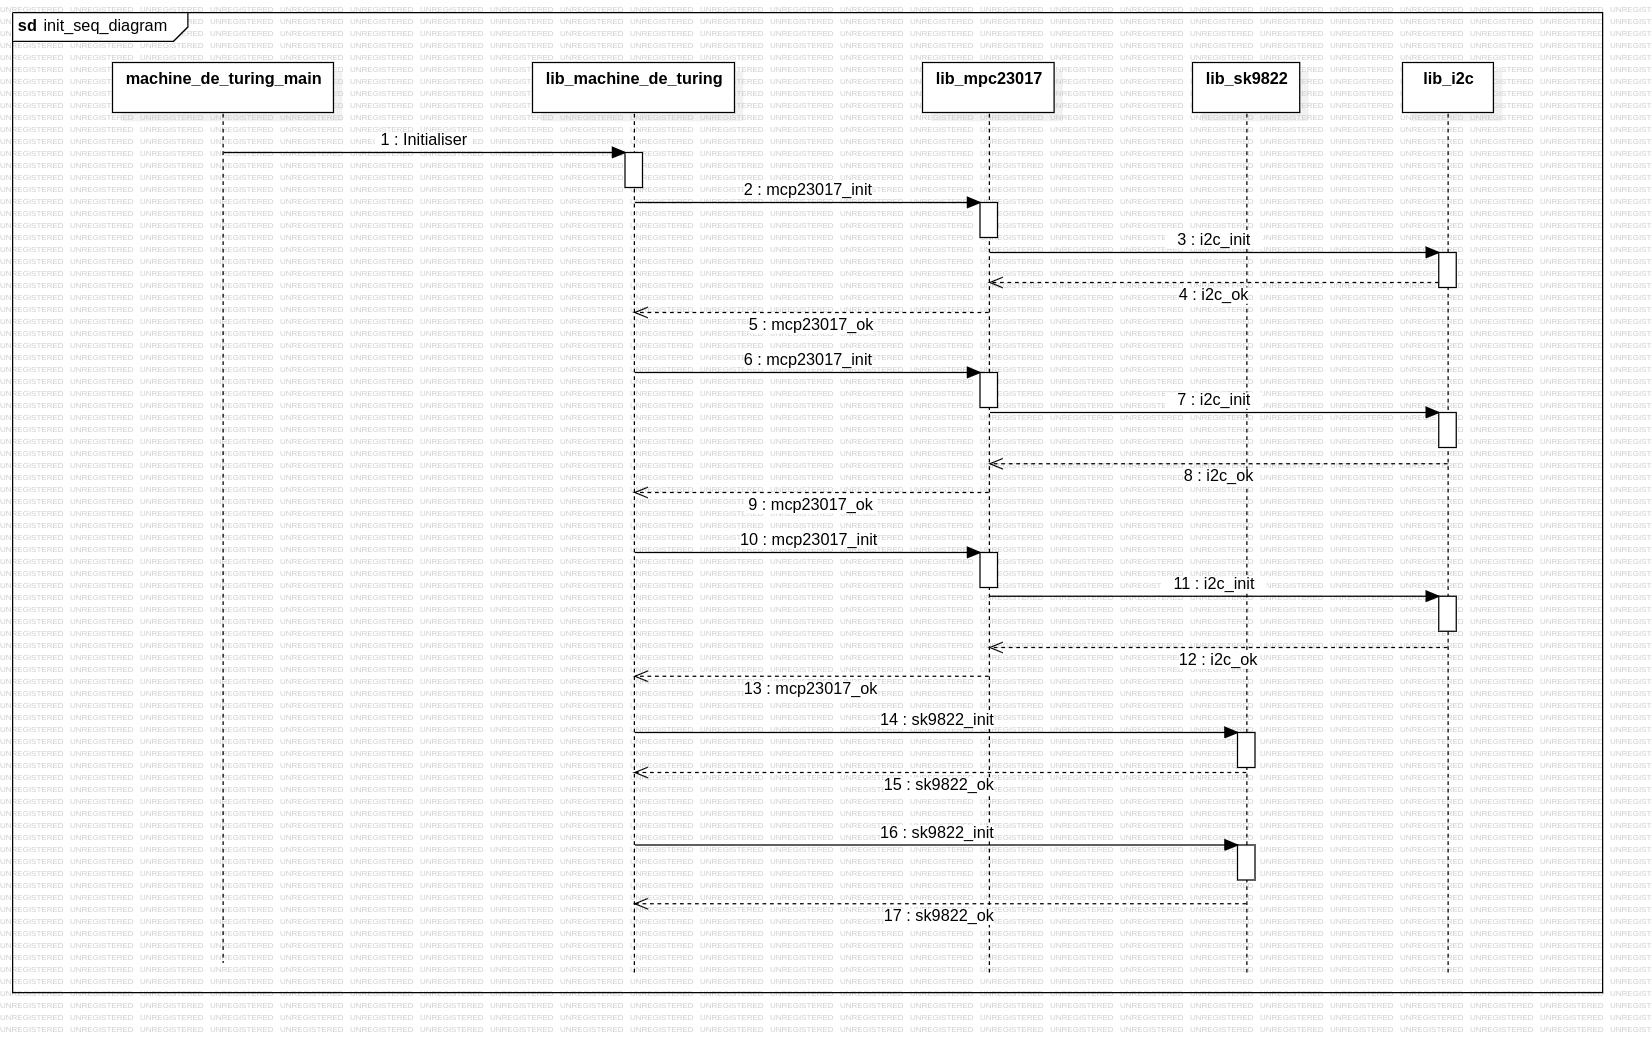
\includegraphics[width=\textwidth]{img/initSeq}
	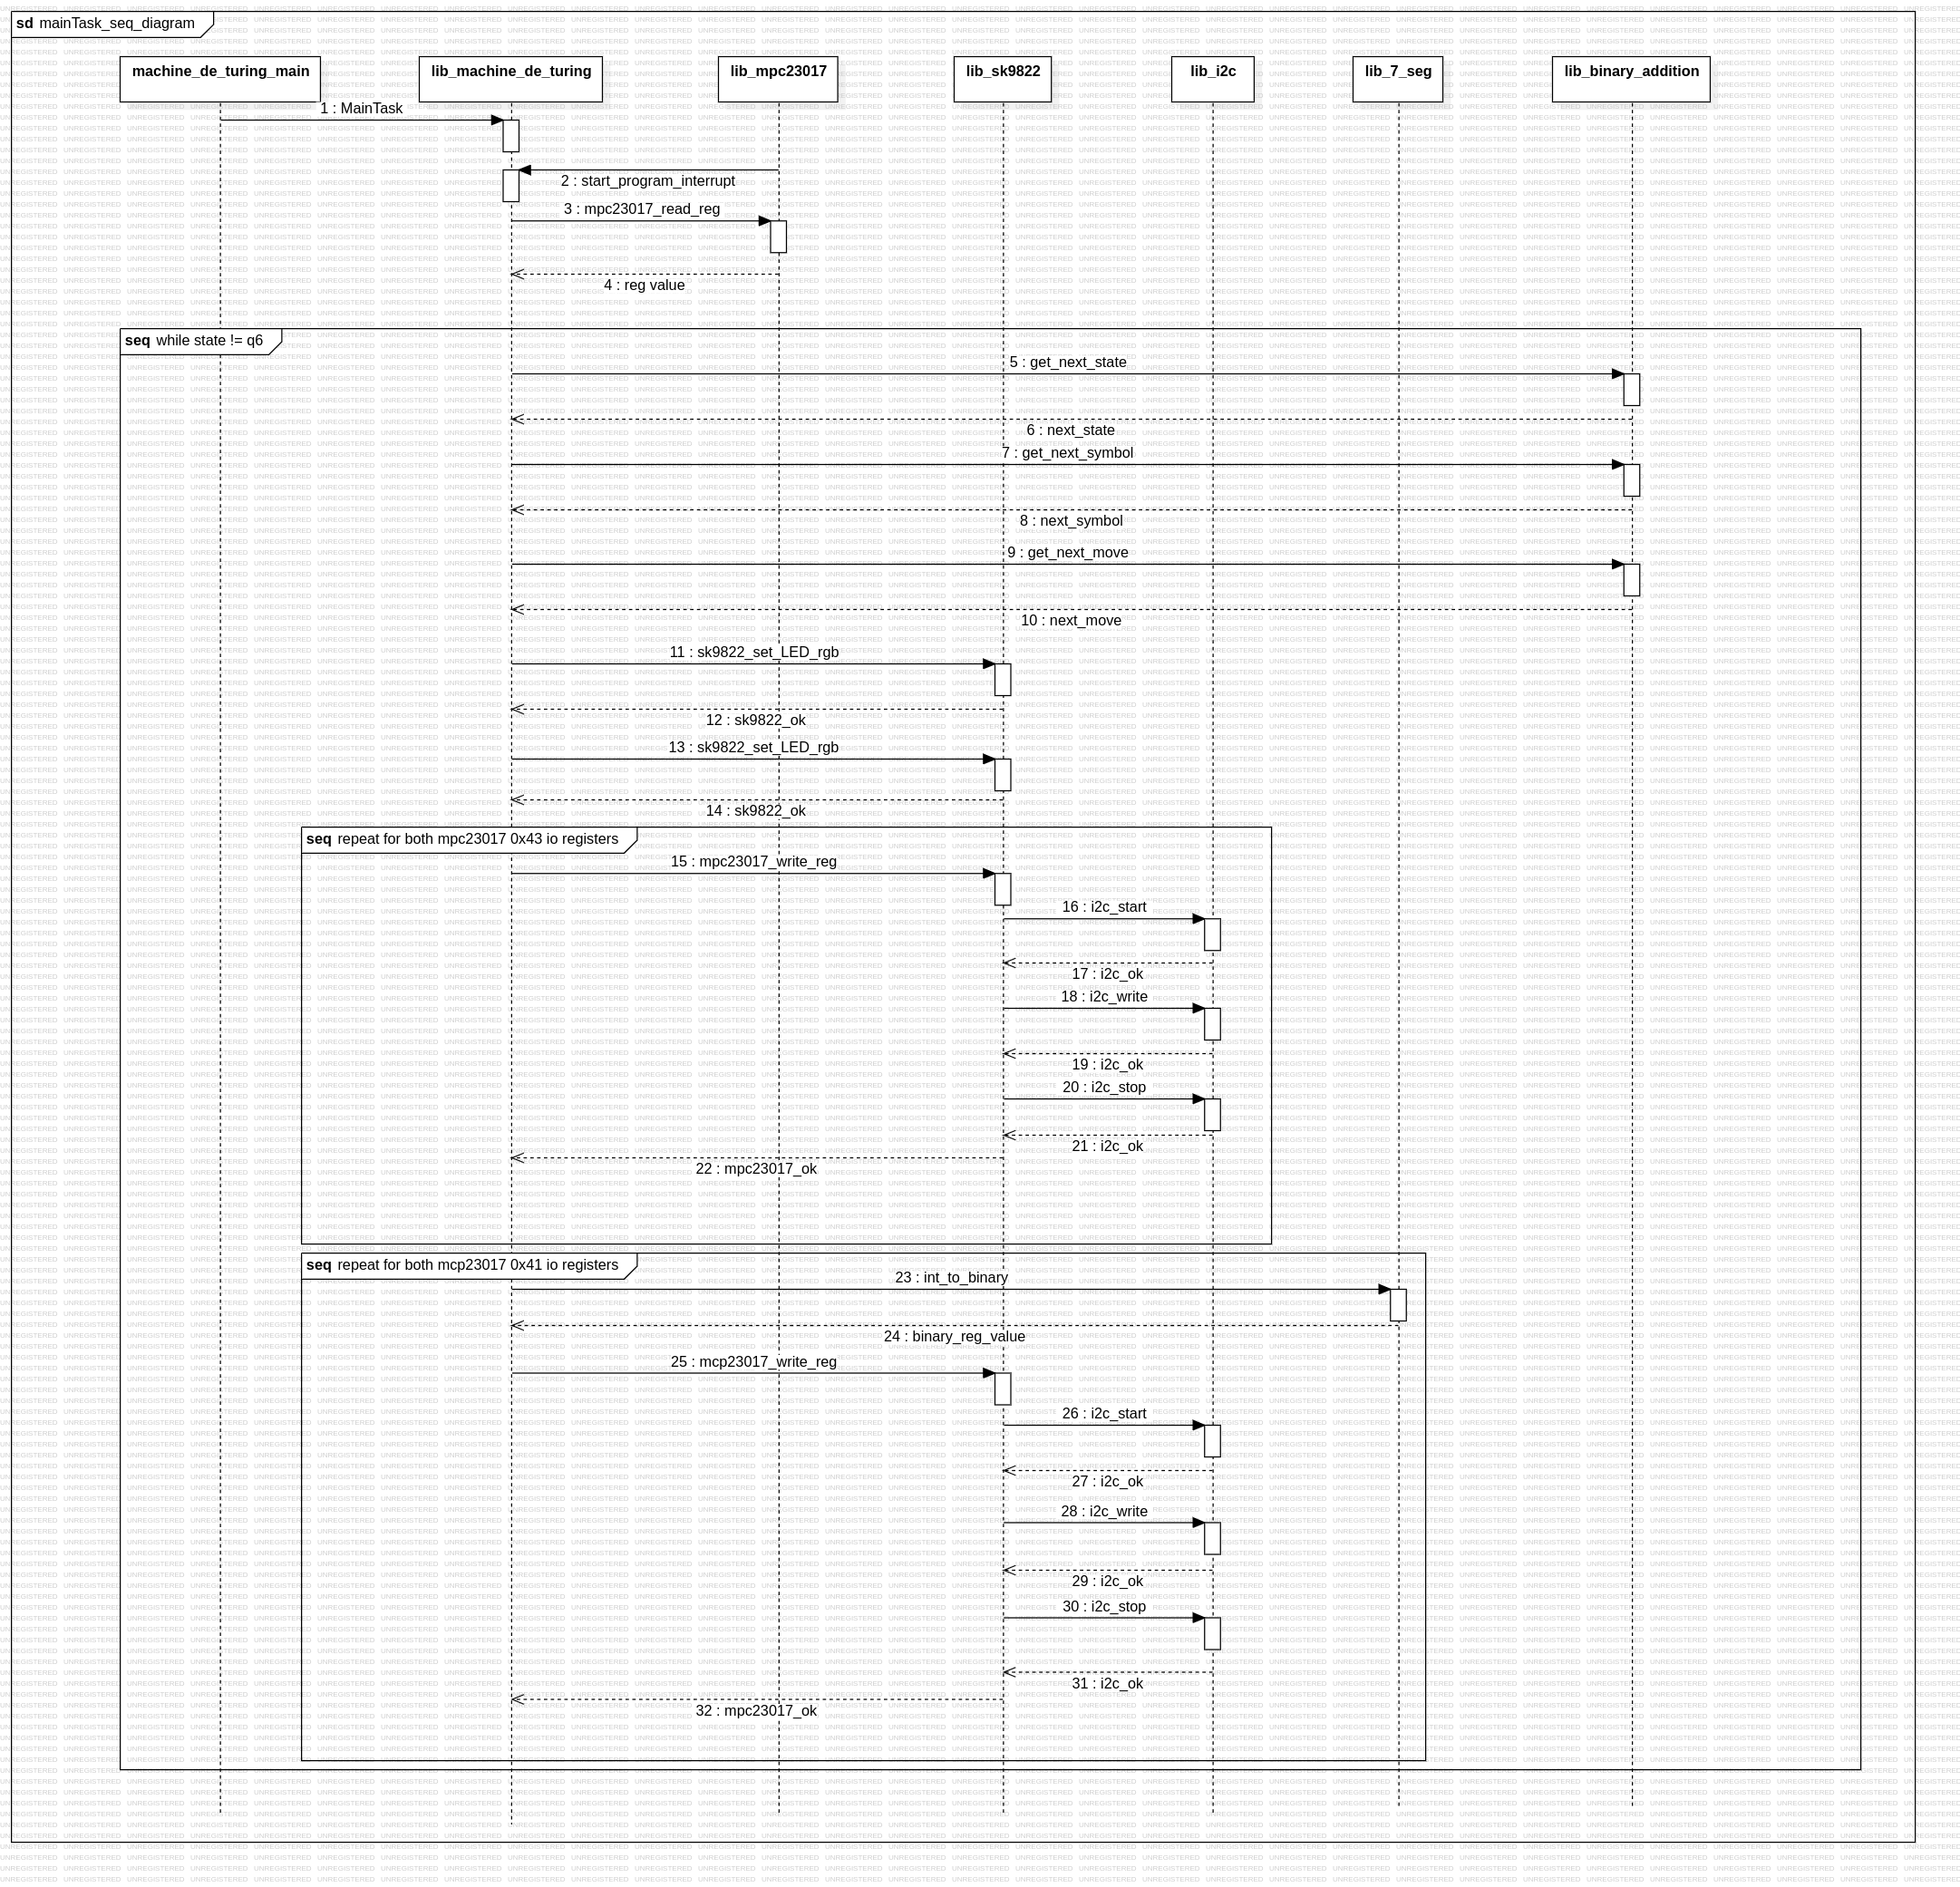
\includegraphics[width=\textwidth]{img/mainTaskSeq}
	\subsection{Algorithme}
	Cet algorithme reprend les deux diagrammes de séquences ci-dessus.
	\begin{lstlisting}
		LIB_MACHINE_DE_TURING
		VARIABLES
			mcp23017_desc_t mpc23017_7_seg
			mcp23017_desc_t mcp23017_bp
			mcp23017_desc_t mcp23017_general
			i2c_desc_t I2CModule
		
		ENUMERATIONS
			mcp23017_err_t
			MCP23017_OK
			MCP23017_ERROR
		
		mcp23017_i2c_init_type_t
			INIT_WITH_I2C1
			INIT_WITH_I2C2
			INIT_ALREADY_DONE
		
		working_mode_t
			MANUAL_MODE
			AUTOMATIC_MODE
		
		STRUCTURES
		mcp23017_desc_t
			i2c_desc_t  *pi2c
			uint8_t     i2c_Address
		
		mcp23017_config_t
			i2c_desc_t  *pi2c;                      
			mcp23017_i2c_init_type_t    initType;   
			uint8_t i2c_Address;
		
		
		machine_de_turing_desc_t
			uint8_t state
			uint8_t symbol
			uint8_t next_state
			uint8_t next_symbol
			uint8_t next_move
		
		CONSTANTES
			MCP23017_7_SEG_ADDRESS      0100001
			MCP23017_BP_ADDRESS         0100010
			MCP23017_GENERAL_ADDRESS    0100011
		
			MCP23017_IOCONA_ADDRESS     0x0A
			MCP23017_IOA_ADDRESS        0x12
			MCP23017_IOB_ADDRESS        0x13
		
		DEBUT
			PROCEDURE Initialiser()
			VARIABLES
				mcp23017_err_t   Res;
				mcp23017_config_t    mcpCfg;
			DEBUT
				Configuration du port B en sortie
		
				// MPC23017 7 segs
				mcpCfg.pi2c = &I2CModule;
				Initialisation avec I2C_1
				Adresse = MCP23017_7_SEG_ADRESS;
		
				Res = mcp23017_init(@mpc23017_7_seg, @mcpCfg)
				SI Res != MCP23017_OK ALORS
					error_handler()
				FIN SI
			
				// MPC23017 BP
				mcpCfg.pi2c = &I2CModule;
				Initialisation avec I2C_1
				Adresse = MCP23017_BP_ADDRESS;
		
				Res = mcp23017_init(@mpc23017_bp, @mcpCfg)
				SI Res != MCP23017_OK ALORS
					error_handler()
				FIN SI
		
				// MPC23017 GENERAL
				mcpCfg.pi2c = &I2CModule;
				Initialisation avec I2C_1
				Adresse = MCP23017_GENERAL_ADDRESS;
		
				Res = mcp23017_init(@mpc23017_bp, @mcpCfg)
				SI Res != MCP23017_OK ALORS
					error_handler()
				FIN SI
		
			FIN Initialiser()
		
			PROCEDURE MainTask()
			VARIABLES
				uint8_t working_mode
				uint8_t next_step
				led_color_t rw_pointer_color
			DEBUT
				Res = mcp23017_read_reg(@mcp23017_bp, MCP23017_IOA_ADDRESS, @working_mode)
				SI Res != MCP23017_OK ALORS
					working_mode = MANUAL_MODE
				FIN SI
		
				TANT QUE mtu->state != ACCEPT_STATE FAIRE
					get_next_state(mtu->state, mtu->symbol, mtu->next_state)
					get_next_symbol(mtu->state, mtu->symbol, mtu->next_symbol)
					get_next_move(mtu->state, mtu->symbol, mtu->next_move)
					set_next_move(mtu->position, mtu->next_move)
		
					sk9822_set_LED_rgb(sk9822_1, mtu->position, mtu->symbol)
					sk9822_set_LED_rgb(sk9822_1, mtu->position, rw_pointer_color)
		
					RegValue = int_to_bin(mtu->state)
					Res = mcp23017_write_reg(@mcp23017_7_seg, MCP23017_IOA_ADDRESS, RegValue)
					SI Res != MCP23017_OK ALORS
						error_handler()
					FIN SI
		
					RegValue = int_to_bin(mtu->next_state)
					Res = mcp23017_write_reg(@mcp23017_7_seg, MCP23017_IOB_ADDRESS, RegValue)
					SI Res != MCP23017_OK ALORS
						error_handler()
					FIN SI
		
					RegValue = generate_general_reg(mtu->symbol, mtu->next_symbol, mtu->next_move)
					Res = mcp23017_write_reg(@mcp23017_general, MCP23017_IOA_ADDRESS, RegValue)
					SI Res != MCP23017_OK ALORS
						error_handler()
					FIN SI
		
					mtu->state = mtu->next_state
					mtu->symbol = mtu->next_symbol
		
					SI working_mode = MANUAL_MODE ALORS
						TANT QUE next_step = 0 FAIRE
						FIN TANT QUE
					SINON
						attendre(2000)
					FIN SI
				FIN TANT QUE
		FIN MainTask()
		
		PROCEDURE error_handler()
			allumer_led()
			TANT QUE 1 FAIRE
		FIN TANT QUE
		FIN error_handler
	\end{lstlisting}
	\subsection{Code}
	Le code ci-dessous implémente, avec quelques différences, l'algorithme précédent :
	\begin{lstlisting}[language=C]
	/**
	* @file    machine_de _turing_main.c
	* @author 	Romain BROUARD
	* @date	2024/05
	* @brief 	main programm of the machine de turing project
	*/
	
	#include "lib_machine_de_turing.h"
	
	#ifndef FCY
	#define FCY 400000UL
	#endif
	
	mcp23017_desc_t mcp23017_7_seg;
	mcp23017_desc_t mcp23017_bp;
	mcp23017_desc_t mcp23017_general;
	i2c_desc_t I2CModule;
	sk9822_desc_t sk9822_symbol;
	sk9822_desc_t sk9822_rw_head;
	machine_de_turing_desc_t *mtu;
	uint8_t next_step = 1;
	
	
	led_color_t red;
	led_color_t green;
	led_color_t lblue;
	
	void Initialiser() {
		mcp23017_err_t   Res;
		mcp23017_config_t    mcpCfg;
		
		TRISB = 0x0000;
		LATB = 0;
		
		mcpCfg.pi2c = &I2CModule;
		mcpCfg.initType = INIT_WITH_I2C1;
		
		// MCP23017 7 segs
		mcpCfg.i2c_Address = MCP23017_7_SEG;
		Res = mcp23017_init(&mcp23017_7_seg,&mcpCfg);
		if (Res != MCP23017_OK) error_handler();
		
		if(mcp23017_write_reg(&mcp23017_7_seg, REG_IOCONA, 0x00) == MCP23017_ERROR) {
			error_handler();
		}
		
		// MCP23017 BP
		mcpCfg.i2c_Address = MCP23017_BP;
		Res = mcp23017_init(&mcp23017_bp,&mcpCfg);
		if (Res != MCP23017_OK) error_handler();
		if(mcp23017_write_reg(&mcp23017_bp, REG_IOCONA, 0x00) == MCP23017_ERROR) {
			error_handler();
		}
		
		// MCP23017 GENERAL
		mcpCfg.i2c_Address = MCP23017_GENERAL;
		Res = mcp23017_init(&mcp23017_general,&mcpCfg);
		if (Res != MCP23017_OK) error_handler();
		if(mcp23017_write_reg(&mcp23017_general, REG_IOCONA, 0x00) == MCP23017_ERROR) {
			error_handler();
		}
		
		red.brightness = 0xFF;
		red.blue = 0;
		red.green = 0;
		red.red = 0xFF;
		
		green.brightness = 0xFF;
		green.blue = 0;
		green.green = 0xFF;
		green.red = 0;
		
		lblue.brightness = 0xFF;
		lblue.blue = 0xE6;
		lblue.green = 0xD8;
		lblue.red = 0xAD;
		
		for(uint8_t i = 0; i<3; i++) {
			sk9822_symbol.led_strip_buff[i] = lblue;
		}
		
		for(uint8_t i = 14; i<N_LED; i++) {
			sk9822_symbol.led_strip_buff[i] = lblue;
		}
		
		sk9822_symbol.led_strip_buff[4] = red;
		sk9822_symbol.led_strip_buff[6] = red;
		sk9822_symbol.led_strip_buff[8] = red;
		sk9822_symbol.led_strip_buff[12] = red;
		sk9822_symbol.led_strip_buff[13] = red;
		sk9822_symbol.led_strip_buff[5] = green;
		sk9822_symbol.led_strip_buff[7] = green;
		sk9822_symbol.led_strip_buff[10] = green;
		sk9822_symbol.led_strip_buff[11] = green;
		
		for(uint8_t i = 0; i<N_LED; i++) {
			sk9822_rw_head.led_strip_buff[i] = lblue;
		}
		sk9822_rw_head.led_strip_buff[13] = red;
		
		mtu->accept = 0;
		mtu->state = 1;
		mtu->next_symbol = RED;
		mtu->position = 12;
	}
	
	void MainTask() {
		uint8_t working_mode;
		uint8_t segValue;
		uint8_t genValue;
		if(mcp23017_read_reg(&mcp23017_bp, REG_GPIOA, &working_mode) == MCP23017_ERROR) {
			working_mode = MANUAL_MODE;
		}
		
		while(!mtu->accept) {
			get_next_transition(mtu);
			
			segValue = int_to_bin(mtu->state);
			if(mcp23017_write_reg(&mcp23017_7_seg, REG_OLATB, segValue) == MCP23017_ERROR) {
				error_handler();
			}
			segValue = int_to_bin(mtu->next_state);
			if(mcp23017_write_reg(&mcp23017_7_seg, REG_OLATA, segValue) == MCP23017_ERROR) {
				error_handler();
			}
			
			genValue = generate_general_reg_value(mtu->symbol, mtu->next_symbol, mtu->next_move);
			if(mcp23017_write_reg(&mcp23017_7_seg, REG_OLATB, segValue) == MCP23017_ERROR) {
				error_handler();
			}
			
			sk9822_rw_head.led_strip_buff[mtu->position] = lblue;
			sk9822_rw_head.led_strip_buff[mtu->next_move] = red;
			mtu->state = mtu->next_state;
			mtu->position = mtu->next_move;
			mtu->symbol = mtu->next_symbol;
			
			if(!working_mode) {
				while(next_step);
			}
			
		}
	}
	
	void error_handler(void){
		LATBbits.LATB15 = 1;
		__delay_ms(500);
	}
	\end{lstlisting}
	\chapter{Synthèse}
	Nous sommes conscient d'avoir vu grand, trop grand. Aujourd'hui, nous pensons avoir une partie d'analyse plutôt solide, nous avons également du code, et nous pensons qu'avec du temps en plus, nous aurions pu arriver à une maquette, au moins de la partie 1. Nous avons manqué de chance vis-à-vis des composants, notamment du ruban de LEDs puisque celui qu'on a reçu ne marche pas.\\
	Nous sommes fiers du travail réalisé, l'analyse est là, les composants sont là, le code est partiellement là, et nous avons pu véritablement mettre en pratique tout ce que nous avons appris en AMIIC et Programmation MCU lors de cette année.\\
	\\
	Ce rapport ne contient pas tous les documents produits, le reste des est disponible dans le dépôt Teams, ou bien sur github, au lien suivant : \url{https://github.com/romain327/machine-turing}. On y trouve notamment les datasheets des composants utilisés, le projet MPLABX contenant les différentes librairies, les schémas structurels, etc.\\
	\chapter{Remerciements}
	Nous remercions Mr. Bocquillon pour nous avoir encadré tout au long de ce projet.\\
	Nous remercions Mr. Rolland pour ses avis et conseils nous ayant permis d'affiner notre analyse.\\
	Nous remercions nos camarades de classe : Lucien, François et Kevin pour avoir répondu à nos questions et nous avoir conseillé.\\
	\chapter{Annexes}
	Ce rapport a été écrit en LaTeX, et la bibliographie réalisée avec BibTeX.
	\section{Connexions minimales recommandées}
	\label{sec:an4.1}
	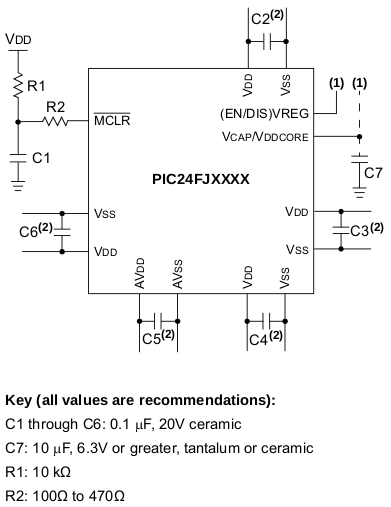
\includegraphics[width=0.7\textwidth]{img/an1}
	\section{Table de transition "Addition de deux nombres binaires"}
	\label{sec:an4.2}
	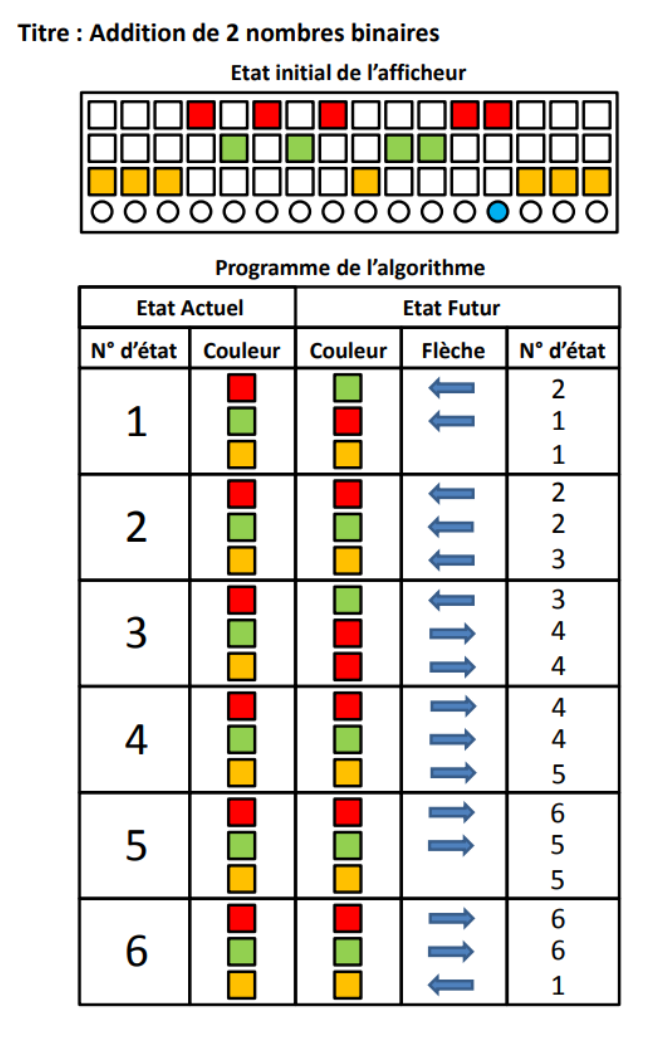
\includegraphics[width=0.9\textwidth]{img/addition_binaire}
	\bibliographystyle{plain}
	\bibliography{biblio}
	
\end{document}